\documentclass{article}
\usepackage[]{url}
\usepackage{graphicx}
\usepackage{hyperref}
\usepackage{mathtools}
\usepackage{tikz}
\usepackage{subcaption}
\usepackage{float}
\usepackage{trimclip}
\usepackage{amsfonts}
\usepackage{pgfgantt}
\begin{document}
\title{Collective motion of squirmers in confined environments\vspace{2cm}}
\author{
M1 CSMI\\
\vspace{3cm}
Roth Robin\\
Supervisors: Van Landeghem Céline, Giraldi Laetitia,\\ Agathe Chouippe
\vspace{2cm}}
\date{August, 2024}
\maketitle

\newpage
\tableofcontents
\newpage
\section{Introduction}
This internship is the continuation of a project realised last semester. The aim of the project was
to develop numerical methods for modeling the dynamics of interacting squirmers. The squirmer is a model for active particles imitating the propulsion of bacteria.\\
A python code to simulate the behaviors of two interacting squirmers has been implemented during the project.\\
These interactions are governed by steric and lubrification forces.
Test cases were conducted to validate our model. Moving forward, we plan to adapt this model to 
simulate interactions among a large number of squirmers.
\section{Context}
The collective behavior of active particles is well studied in the literature. 
Various models exist to simulate these active particles, such as the Vicsek model\cite{Vicsek} and the Squirmer model. \\
The squirmer model initially proposed by Lighthill in 1952\cite{Wikipedia}, represents a spherical Stokesian swimmer with a surface that undergoes 
small-amplitude deformations to achieve propulsion. 
This model has been applied to a range of microswimmer dynamics in both biological and artificial contexts. 
Blake\cite{Wikipedia} later refined the model, adapting it to describe a spherical microswimmer
 covered with a dense array of beating cilia. Instead of representing individual cilia, the model uses a continuous, deformable layer 
 that propagates the wave.\\
The aim of this internship is to study squirmers, 
in a confined domain and to compare their collective motion with that of the active particles using the Vicsek model. 
The motion of the squirmers is described by a continuous model that approximates lubrification and 
steric forces\cite{Brumley}\cite{Lauga}.

\section{Objectives}
The main goal is to model the dynamics of a group of squirmers within confined environments and to
 study the influence of numerical parameters on their collective behavior.\\
 To achieve this objective, the following tasks will be carried out:
 \begin{itemize}
     \item Validate the formulas of the steric and lubrification forces from the previous project.
     \item Investigate the impact of altering the parameter $\beta$, which defines the
    type of squirmers (pusher, puller, neutral swimmer), on the interaction between two squirmers.
     \item Conduct a comparative analysis of the interaction between a squirmer and a 
    boundary of the domain by varying the initial angle of the squirmer and the parameter $\beta$, 
    to comprehensively understand their influence on the system dynamics.
     \item Update and vectorize the code to enable a simulation of a larger number of squirmers.
     \item Examine the impact of numerical parameters on the collective behavior of squirmers.
\end{itemize}
All of these steps are consolidated in the following roadmap:
\begin{center}
    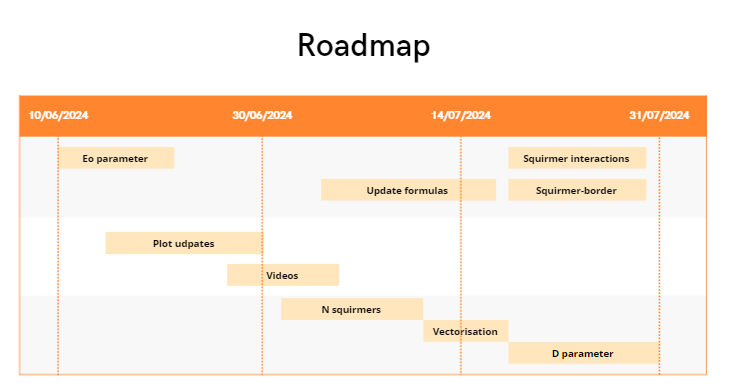
\includegraphics[width=1.2\textwidth]{Presentation/images/roadmap_stage.png}
\end{center}

\newpage
\section{Vicsek model}
In this section a detailed overview of the Vicsek model will be provided.
\begin{center}
    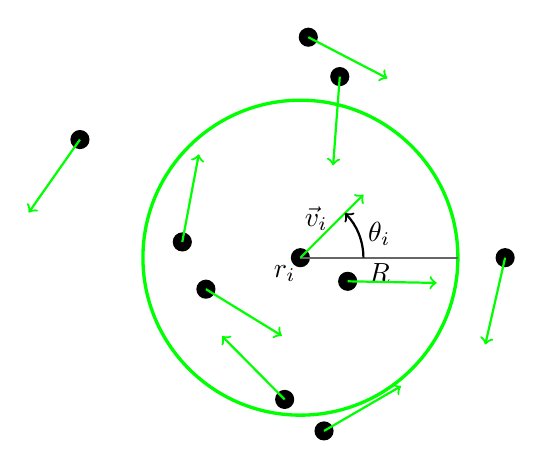
\begin{tikzpicture}
        \draw[color=green, very thick](0,0) circle (2);
        \node at (-0.2,-0.2) {{$r_i$}};
        \filldraw[color=black, fill=black, very thick](0,0) circle(0.1);
        \filldraw[color=black, fill=black, very thick](-1.5,0.2) circle(0.1);
        \filldraw[color=black, fill=black, very thick](0.5,2.3) circle(0.1);
        \filldraw[color=black, fill=black, very thick](2.6,0) circle(0.1);
        \filldraw[color=black, fill=black, very thick](-0.2,-1.8) circle(0.1);
        \filldraw[color=black, fill=black, very thick](0.6,-0.3) circle(0.1);
        \filldraw[color=black, fill=black, very thick](-1.2,-0.4) circle(0.1);
        \filldraw[color=black, fill=black, very thick](-2.8,1.5) circle(0.1);
        \filldraw[color=black, fill=black, very thick](0.3,-2.2) circle(0.1);
        \filldraw[color=black, fill=black, very thick](0.1,2.8) circle(0.1);
        \draw[thick, -, color=black!60] (0,0) -- (2,0);
        \node at (1,-0.2) {{$R$}};
        %Length of the arrow
        \pgfmathsetmacro{\len}{sqrt(1.28)}

        %Draw arrows with random directions
        \foreach \x/\y in {-1.5/0.2, 0.5/2.3, 2.6/0, -0.2/-1.8, -1.2/-0.4, -2.8/1.5, 0.3/-2.2, 0.1/2.8} {
            \pgfmathsetmacro{\angle}{random()*360}
            \draw[thick, ->, color=green] (\x,\y) -- ++({\len*cos(\angle)},{\len*sin(\angle)});
        }
        \draw[thick, ->, color=green] (0,0) -- (0.8,0.8);
        \draw[thick, ->, color=green] (0.6, -0.3) -- ++ ({\len*cos(-1.04)},{\len*sin(-1.04)});
        \node [color=black] at (0.2,0.5) {{$\vec{v}_i$}};
        \draw[thick, ->, color=black] (0.8, 0) arc (0:45:0.8);
        \node at (1, 0.3) {{$\theta_i$}};
    \end{tikzpicture}
\end{center}

The Vicsek model consists of $N$ particles with $r_i(t)$ in $\mathbb{R}^2$ and $\theta_i(t) \in \left[0, 2\pi\right]$ 
their mass center and orientations.\\
All particles have the same velocity $v_0$ and radius.
The evolution of the orientation $\theta_i(t)$ at each time step $\Delta t$ is given by:
$$\theta_i(t + \Delta t) = \langle\theta_j(t)\rangle_{|r_i(t) - r_j(t)| < R} + \epsilon_i(t),$$
with
$$\langle\theta_j(t)\rangle = \arctan\left(\frac{\sin(\theta_j(t))}{\cos(\theta_j(t))}\right).$$
$R$ is the range of interaction, $\langle\theta_j(t)\rangle_{|r_i(t) - r_j(t)| < R}$ the average 
orientation of the particles in the range $R$ of
 the $i$-th particle (including itself) at the time $t$ and $\epsilon_i(t)$ represents the noise. 
 It is a random number taken from a uniform probability distribution
over $\left(-\frac{\eta}{2}, \frac{\eta}{2}\right)$ where $\eta$ is the main tool that counteracts the alignment of the particles.\\
\\
The evolution of the position $r_i(t)$ at each time step $\Delta t$ is described by:
$$ r_i(t + \nabla t) = r_i(t) + v_0\Delta t \begin{pmatrix}
    \cos(\theta_i(t))\\
    \sin(\theta_i(t))
\end{pmatrix}.$$
The velocity $\vec{v}_i(t)$ is defined by:
$$\vec{v}_i(t) = v_0\begin{pmatrix}
    \cos\theta_i(t)\\
    \sin\theta_i(t)
\end{pmatrix}.$$
The collective behavior of the particles are quantified by the polar order parameter $v_a$ which is given by:
$$v_a = \frac{1}{Nv_0}\left|\sum^{N}_{i=1}\vec{v}_i\right|.$$
The boundary conditions are reflective, if a particle is outside of the domain after computing $r_i(t + \Delta t)$, the new 
coordinates and orientations of the particle are given by:\\
For the x-boundary:
$$|x_i(t + \Delta t)| = 2L_x - |x_i(t + \Delta t)|,$$
$$\theta_{i}(t + \Delta t) = \pi - \theta_i(t + \Delta t).$$
For the y-boundary:
$$|y_i(t + \Delta t)| = 2L_y - |y_i(t + \Delta t)|,$$
$$\theta_i(t + \Delta t) = -\theta_i(t + \Delta t).$$
Where $L_x$ represents the length of the domain, and $L_y$ represents the width of the domain.
\begin{center}
    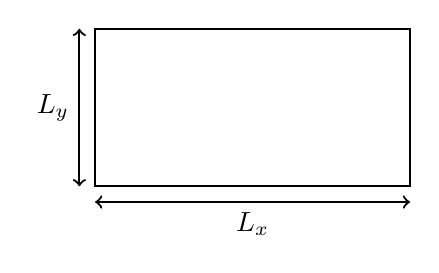
\begin{tikzpicture}
        \draw[thick] (0,0) -- (4,0) -- (4,2) -- (0,2) -- cycle;
        \draw[<->,thick] (-0.2,0) -- (-0.2,2) node[midway,left] {$L_y$};
        \draw[<->,thick] (0,-0.2) -- (4,-0.2) node[midway,below] {$L_x$};
    \end{tikzpicture}
\end{center}
These conditions ensures that the particles reflect off the boundaries.
We will compare our results with those obtained using a similar model.

\newpage
\section{Squirmer model}
I will continue by detailing the squirmer model as well as the interactions 
between such active particles. This model uses lubrification forces 
and torques to describe particle behavior, while the Vicsek model focuses more
on collective behavior to model particle movement.

\begin{center}
   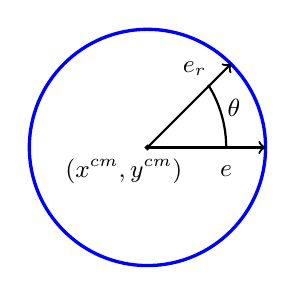
\begin{tikzpicture}
      \small
      
      \draw[color=blue, very thick](2.5,2.5) circle (1.5);
      
      \draw[color=black, very thick](2.5,2.5) circle (0.01);
      
      \node  at (2.5-0.3,2.5-0.3) {{$(x^{cm},y^{cm})$}};
      
      \draw[thick, ->] (2.5,2.5) -- (4,2.5);
      \node  at (3.5,2.2) {{$e$}};
   
      \pgfmathsetmacro{\xcoord}{2.5 + 1.5*cos(45)}
       \pgfmathsetmacro{\ycoord}{2.5 + 1.5*sin(45)}
       \draw[thick, ->] (2.5,2.5) -- (\xcoord,\ycoord);
      \node  at (3.1,3.5) {{$e_r$}}; 
      \draw[thick, -] (3.5,2.5) arc[start angle=0, end angle=32, radius=1.5];
      \node at (3.6,3) {${\theta}$}; 
      
         
      \end{tikzpicture}
    \end{center}
The time-independent velocity $u$ defined on the surface of the squirmer is given 
in polar coordinates by :

\begin{align*}
   \left\{\begin{array}{rcl}
      u_r(R,\theta) &=& 0 \\
      u_\theta(R,\theta) &=& B_1\mathrm{sin}(\theta)+B_2\mathrm{sin}(\theta)\mathrm{cos}(\theta)
   \end{array}\right.\ \cite{Lauga};
\end{align*}

With $R$ denoting the particle's radius, and $B_1$ and $B_2$ being constants. By setting $\beta=\frac{B_2}{B_1}$, we have :
$$
u_\theta(R,\theta) = B_1(\mathrm{sin}(\theta) + \beta \mathrm{sin}(\theta)\mathrm{cos}(\theta)),
$$
where $\beta$ is the type of the squirmer :
$$\left\{
    \begin{array}{ll}
        \beta = 0 : \text{neutral swimmer}  \\
        \beta < 0 : \mathrm{pusher} \\
        \beta > 0 : \mathrm{puller} \\
    \end{array}
\right.$$
and $B_1$ describes the swimming velocity $v_0 = \frac{2 B_1}{3}$.
\\ Now let us put $u$ in cartesian coordinates :
\begin{align*}
    u &= \begin{pmatrix}
   u_x \\
   u_y
\end{pmatrix}
= \begin{pmatrix}
   \mathrm{cos}(\theta) & -\mathrm{sin}(\theta) \\
   \mathrm{sin}(\theta) & \mathrm{cos}(\theta)
\end{pmatrix}
\begin{pmatrix}
   u_r \\
   u_\theta
\end{pmatrix}, \\
&= B_1 (1 + \beta \mathrm{cos}(\theta))
\begin{pmatrix}
   -\mathrm{sin}^2(\theta) \\
   \mathrm{sin}(\theta)\mathrm{cos}(\theta)
\end{pmatrix}.
\end{align*}

We define $e_r$ the unit vector pointing from the center to the surface 
$$
e_r = \begin{pmatrix}
   \frac{x - x^{cm}}{R}  \\
   \frac{y - y^{cm}}{R} 
\end{pmatrix} = \begin{pmatrix}
   \mathrm{cos}(\phi) \\
   \mathrm{sin}(\phi)
\end{pmatrix}$$ 

and $e$ = 
$\begin{pmatrix}
   \mathrm{cos}(\theta) \\
   \mathrm{sin}(\theta) \end{pmatrix}$ the swimming direction of the squirmer. 
   
   By fixing $\theta$ = 0, one has $e$ = $\begin{pmatrix}
   1 \\
   0 \end{pmatrix}$ and one finds the following expression for the velocity field 
   in cartesian coordinates: 

\begin{align*}
u &= B_1 \left(1+\beta \mathrm{cos}(\theta) \right) \begin{pmatrix}
   -\mathrm{sin}^2(\theta) \\
   \mathrm{sin}(\theta)\mathrm{cos}(\theta)
\end{pmatrix},  \\
&= B_1 \left(1+\beta \mathrm{cos}(\theta) \right) \begin{pmatrix}
   \mathrm{cos}^2(\theta)-1 \\
   \mathrm{sin}(\theta)\mathrm{cos}(\theta)
\end{pmatrix}, \\
&= B_1 \left(1+\beta \begin{pmatrix}
   1 \\
   0 \end{pmatrix}\begin{pmatrix}
   \mathrm{cos}(\theta) \\
   \mathrm{sin}(\theta)
\end{pmatrix}\right) \left[ \left( \begin{pmatrix}
   1 \\
   0 \end{pmatrix}\begin{pmatrix}
   \mathrm{cos}(\theta) \\
   \mathrm{sin}(\theta)
\end{pmatrix}\right) \begin{pmatrix}
   \mathrm{cos}(\theta) \\
   \mathrm{sin}(\theta)
\end{pmatrix} - \begin{pmatrix}
   1 \\
   0 \end{pmatrix}\right], \\
&= B_1(1+\beta (e \cdot e_r)) [(e \cdot e_r)e_r - e]. 
\end{align*}

\vspace{0.5 cm}
Thus, $u$ in cartesian coordinates is given by :
\begin{equation*}
\boxed{u_r = B_1(1+\beta (e\cdot e_r)) [(e\cdot e_r)e_r - e].}
\end{equation*}


\section{Dynamics of two interacting squirmers}
\subsection{The evolution of the mass center}
The evolution of the mass center $r_i$ = $(X_i, Y_i)$ of one squirmer $i$ in presence of 
another squirmer $j$ and rigid boundaries, is given by the Langevin equation:
\begin{center}
$\boxed{\frac{dr_i}{dt}$ = $v_0 p_i -  \sum\limits_{i \ne j}\nabla_{r_{ij}} V_{ij} - \sum\limits_{i}\nabla_{r_i} V_i + \sum\limits_{i\ne j}\left[F_{i(j)\rightarrow i} + F_{j(i)\rightarrow i}\right]+ \sum\limits_{k \in w}F_{k\rightarrow i}^w + \sqrt{2D}\eta_i(t)}$
\end{center}
We have : \begin{itemize}
    \item $v_0$ the particle velocity,
    \item $p_i$ = $(\mathrm{cos}(\theta),\mathrm{sin}(\theta))^T$ orientation,
    \item $F_{i(j)\rightarrow k}$ the lubrification forces applied on the $k^{th}$ squirmer and generated by the $i^{th}$ squirmer in presence of the $j^{th}$ one \cite{Brumley},
    \item $F^w_{k\rightarrow i}$ the lubrification forces exerted on the $i^{th}$ squirmer due to the presence of the $k^{th}$ wall\cite{Brumley},
    \item $V_{ij}$ and $V_i$ are the Weeks-Chandler-Andersen potential use to define a repulsive steric force avoiding 
    the overlapping of two squirmers or of one squirmer and a rigid boundary. 
    The force is activated when the distance between two surfaces is small,
    \item $D$ the translational diffusivity,
    \item $\eta_i$ are independent noises. 
\end{itemize} 
\vspace{0,5cm}
The second law of Newton states\cite{Newton}:
$$m\vec{a} = \sum\limits_i \vec{F}_i.$$
The force of viscosity on a small sphere moving through a viscous fluid is given by the Stokes-Einstein relation\cite{Stokes}:
$$F_d = 6\mu\pi Rv_0\frac{dr_i}{dt}.$$
We consider the squirmers propulsion in absence of inertia: $m\vec{a} = 0$. Hence one has:
$$0 = -F_d + \sum\limits_{i \ne d} F_i,$$
we have:
$$\frac{dr_i}{dt} = \frac{1}{6\mu\pi R}\sum\limits_{i \ne d} F_i.$$
The Weeks-Chandler-Andersen potential is given by:
$V_{ij}$ = $\frac{E_s}{6\pi\mu R}\left[\left(\frac{2R}{\lvert r_{ij}\rvert}\right)^{12} - \left(\frac{2R}{\lvert r_{ij}\rvert}\right)^6\right]$ and  $V_i$ = $\frac{E_s}{6\pi\mu R} \left[ \left( \frac{R}{\lvert r - r_i \rvert} \right)^{12} - \left( \frac{R}{\lvert r - r_i \rvert} \right) ^6 \right]$ 
\vspace{0,3cm}
\\With : \begin{itemize}
    \item $r_{ij}$ = $\sqrt{D_x^2+D_y^2}$, $\lvert r_{ij} \rvert$ the distance between the centers of two squirmers,
    \item $\lvert r - r_i\rvert$ the distance between the wall and the squirmer center,
    \item $E_s$ a positive constant,
    \item $R$ the radius of a squirmer,
    \item $\mu$ the dynamic viscosity.
\end{itemize}

\vspace{0,5cm}
We want to compute the steric force applied between two squirmers, given by $\nabla_{r_{ij}} V_{ij}$:

\begin{align*}
\frac{\partial V_{ij}}{\partial D_x} &= \frac{\partial}{\partial D_x}\frac{E_s}{6\pi\mu R}\left[\left(\frac{2R}{\lvert r_{ij}\rvert}\right)^{12} - \left(\frac{2R}{\lvert r_{ij}\rvert}\right)^6\right] \\
&= \frac{E_s}{6\pi\mu R} \left[\frac{\partial}{\partial D_x}\left(\frac{2R}{\lvert r_{ij}\rvert}\right)^{12} - \frac{\partial}{\partial D_x} \left(\frac{2R}{\lvert r_{ij}\rvert}\right)^6\right] \\
&= \frac{E_s}{6\pi\mu R} \left[ \frac{-12 D_x (2R)^{12}(r_{ij})^{10}}{(r_{ij})^{24}} - \frac{-6D_x(2R)^6(r_{ij})^4}{(r_{ij})^{12}}  \right] \\
&= \frac{-12 E_s}{2r6\pi\mu R} \left[ \frac{D_x (2R)^{13}}{(r_{ij})^{14}} - \frac{D_x (2R)^{7}}{2(r_{ij})^8}\right] \\
&= -\frac{E_s}{2R^2\pi\mu} \frac{D_x}{r_{ij}} \left[ \frac{2(2R)^{13}}{(r_{ij})^{13}} - \frac{(2R)^7}{(r_{ij})^{7}}\right].
\end{align*}
Equivalently, we have : 
$\frac{\partial V_{ij}}{\partial D_y}$ = $-\frac{E_s}{2R^2\pi\mu} \frac{D_y}{r_{ij}}\left[ \frac{2(2R)^{13}}{(r_{ij})^{13}} - \frac{(2R)^7}{(r_{ij})^7} \right].$
\\ We find : 
\begin{equation*}
    \boxed{\nabla_{r_{ij}} V_{ij} = 
    \begin{pmatrix}
        -\frac{E_s}{2R^2\pi\mu} \frac{D_x}{r_{ij}}\left[ \frac{2(2R)^{13}}{(r_{ij})^{13}} - \frac{(2R)^7}{(r_{ij})^7} \right] \\
        -\frac{E_s}{2R^2\pi\mu} \frac{D_y}{r_{ij}}\left[ \frac{2(2R)^{13}}{(r_{ij})^{13}} - \frac{(2R)^7}{(r_{ij})^7} \right]
    \end{pmatrix}}
\end{equation*}

\vspace{0,5cm}

In addition, we need to compute $\partial_{r_i} V_i$ to obtain the force applied between a squirmer and a rigid boundary.

\begin{align*}
    \frac{\partial V_i}{\partial X} &= \frac{\partial}{\partial X} \left( \frac{E_s}{6\pi\mu R} \left[ \left( \frac{R}{\lvert r - r_i \rvert} \right)^{12} - \left( \frac{R}{\lvert r - r_i \rvert} \right) ^6 \right] \right) \\
    &= \frac{\partial}{\partial X} \left( \frac{E_s}{6\pi\mu R} \left[ \left( \frac{R}{\sqrt{( X_{box}-X)^2 + (Y_{box}-Y)^2}} \right)^{12} - \left( \frac{R}{\sqrt{( X_{box}-X)^2 + (Y_{box}-Y)^2}} \right) ^6 \right] \right) \\
    &= \frac{E_s}{6\pi\mu R}\left[ 12(X_{box}-X)\frac{R^{12}}{\lvert r - r_i\rvert^{14}} - 6(X_{box}-X)\frac{R^6}{\lvert r-r_i\rvert^8} \right] \\
    &= -\frac{E_s (X_{box}-X)}{\pi\mu R^2 \lvert r - r_i \rvert } \left[ 2 \left( \frac{R}{\lvert r-r_i\rvert} \right)^{13} - \left( \frac{R}{\lvert r-r_i\rvert}\right)^7 \right].
\end{align*}
Equivalently, we have : $\frac{\partial V_i}{\partial Y}$ = $ - \frac{E_s (Y_{box}-Y)}{\pi\mu R^2 \lvert r - r_i \rvert } \left[ 2 \left( \frac{R}{\lvert r-r_i\rvert} \right)^{13} - \left( \frac{R}{\lvert r-r_i\rvert}\right)^7 \right].$

We have : 
\begin{equation*}
    \boxed{\nabla_{r_i} V_i = \begin{pmatrix}
        - \frac{E_s (X_{box}-X)}{\pi\mu R^2 \lvert r - r_i \rvert } \left[ 2 \left( \frac{R}{\lvert r-r_i\rvert} \right)^{13} - \left( \frac{R}{\lvert r-r_i\rvert}\right)^7 \right] \\
        - \frac{E_s (Y_{box}-Y)}{\pi\mu R^2 \lvert r - r_i \rvert } \left[ 2 \left( \frac{R}{\lvert r-r_i\rvert} \right)^{13} - \left( \frac{R}{\lvert r-r_i\rvert}\right)^7 \right]
    \end{pmatrix}}
\end{equation*}
These steric forces are applied on two squirmers when $r_{ij} < R2^{\frac{7}{6}}$.

\begin{center}
   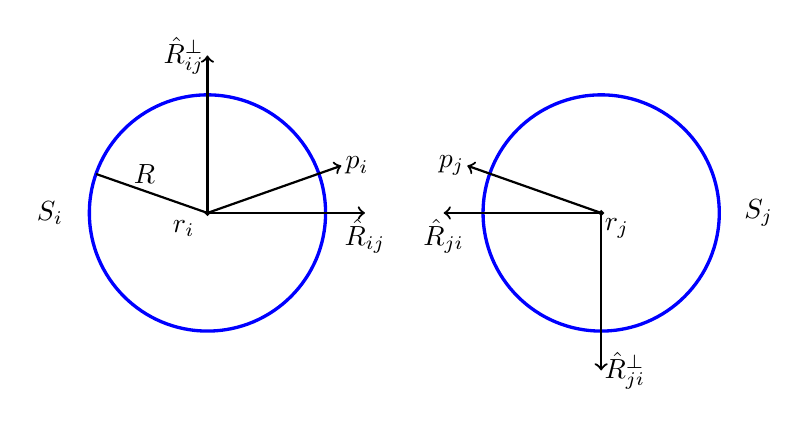
\begin{tikzpicture}
   
   \draw[color=blue, very thick](5,5) circle (1.5);
   \draw[color=blue, very thick](0,5) circle (1.5);
   
   \draw[color=black, very thick](0,5) circle (0.01);
   \draw[color=black, very thick](5,5) circle (0.01);
   
   \node  at (-0.3,5-0.2) {{$r_i$}};
   \node  at (5+0.2,5-0.2) {{$r_j$}};
   
   \node  at (-2,5) {{$S_i$}};
   \node  at (7,5) {{$S_j$}};
   
   \draw[thick, ->] (0,5) -- (1.7,5+0.6);
   \draw[thick, ->] (5,5) -- (5-1.7,5+0.6);
   
   \node  at (1.9,5+0.6) {{$p_i$}};
   \node  at (5-1.9,5+0.6) {{$p_j$}};
   
   \draw[thick] (0,5) -- ({-cos(45)*2}, {5+0.7*sin(45)});
   \node  at (-0.8,5+0.5) {{$R$}};
   
   \draw[thick, ->] (0,5) -- (2,5);
   \draw[thick, ->] (5,5) -- (3,5);
   
   \node  at (2,5-0.3) {{$\hat{R}_{ij}$}};
   \node  at (3,5-0.3) {{$\hat{R}_{ji}$}};
   
   \draw[thick, ->] (0,5) -- (0,7);
   \node  at (-0.3,7) {$\hat{R}_{ij}^{\perp}$};
   
   
   \draw[thick, ->] (5,5) -- (5,3);
   \node  at (5.3,3) {$\hat{R}_{ji}^{\perp}$};
   
   \end{tikzpicture}
   \end{center}
The figure shows the different vectors involved in the computations which will follow.
\\We define: 
\begin{itemize}
    \item $W_n(x)$ = $\frac{2}{n(n+1)}P_n'(x)$ \cite{Brumley},
    \item $P_n(x)$ the Legendre polynomials \cite{Wikipedia} given by:
    \begin{itemize}
        \item $P_1(x) = x,$
        \item $P_2(x) = \frac{1}{2}(3x^2-1),$
    \end{itemize}
    \item $p_i = (\cos\theta_i, \sin\theta_i),$
    \item $\hat{R}_{ij} = \frac{r_{ij}}{\left|r_{ij}\right|}$,
    \item $\hat{R}^{\perp}_{ij} = rot(\frac{\pi}{2})\hat{R}_{ij}.$
\end{itemize}

The tangential lubrication forces acting on the two spheres, depending on the direction of the vectors $\hat{R}_{ij}$ and $\hat{R}^{\perp}_{ij}$, are defined by\cite{Brumley}:
\\ 
\footnotesize
$F_{i(j)\rightarrow i}^{y}$ = $9 \mu \pi R \frac{\lambda ^2}{(\lambda +1)^2} \sum_{n} \left[ B_n W_n(p_i\hat{R}_{ij})(-p_i\hat{R}_{ij}) + \frac{1}{2} B_n W_n'(p_i\hat{R}_{ij})(p_i\hat{R}^{\perp}_{ij})^2 \right] (ln \epsilon + O(1)).$
\normalsize
For $n$ = 1 : \begin{align*}
    W_1(p_i\hat{R}_{ij}) &= 1, \\
    W_1'(p_i\hat{R}_{ij}) &= 0, \\
    -B_1 W_1(p_i\hat{R}_{ij})p_i\hat{R}_{ij} + \frac{1}{2} B_1  W_1'(p_i\hat{R}_{ij}) (p_i\hat{R}^{\perp}_{ij})^2  &= -B_1 p_i\hat{R}_{ij}.
\end{align*} 
For $n$ = 2 : \begin{align*}
    W_2(p_i\hat{R}_{ij}) &= p_i\hat{R}_{ij}, \\
    W_2'(p_i\hat{R}_{ij}) &= 1,\\
    -B_2 W_2(p_i\hat{R}_{ij})p_i\hat{R}_{ij}+ \frac{1}{2} B_2  W_2'(p_i\hat{R}_{ij}) (p_i\hat{R}^{\perp}_{ij})^2  &= -B_2 (p_i\hat{R}_{ij})^2 + \frac{1}{2} B_2(p_i\hat{R}^{\perp}_{ij})^2.
\end{align*}  

Since all squirmers share the same radius $R$, we have $B_1 = \frac{3}{2}v_0$, $B_2 = B_1\cdot\beta$ and $\lambda=1$, so:
\begin{align*}
\footnotesize
6\mu\pi RF_{i(j)\rightarrow i}^{y} = 9 \mu \pi R \frac{\lambda ^2}{(\lambda +1)^2} \left[ -B_1 p_i\hat{R}_{ij} -B_2 (p_i\hat{R}_{ij})^2 + \frac{1}{2} B_2(p_i\hat{R}^{\perp}_{ij})^2\right](ln \epsilon + O(1))\\
= 9 \mu \pi R \frac{1}{4}\cdot\frac{3}{2}v_0\left[ -p_i\hat{R}_{ij} -\beta (p_i\hat{R}_{ij})^2 + \frac{1}{2} \beta(p_i\hat{R}^{\perp}_{ij})^2\right](ln \epsilon + O(1))
\end{align*}
\begin{equation*}
\boxed{
    F_{i(j)\rightarrow i}^{y} = -\frac{9}{16}v_0
\left[(p_i\hat{R}_{ij})(1 + \beta p_i\hat{R}_{ij}) - \frac{1}{2}\beta(p_i\hat{R}^{\perp}_{ij})^2\right](ln \epsilon + O(1))
}
\end{equation*}
\normalsize
\vspace{0.5cm}

The normal forces acting on the two spheres can be calculated explicitly by\cite{Brumley}:
\begin{center}
    $F_{i(j)\rightarrow i}^{x}$ = $-\frac{4}{5} \mu \pi R \frac{\lambda(\lambda +4)}{(\lambda +1)^2} \sum_{n} B_n W_n(p_i\hat{R}_{ij}) (ln \epsilon + O(1))$
\end{center}
 So :
\begin{align*}
    \footnotesize
    6\mu\pi RF_{i(j)\rightarrow i}^{x} = -\frac{4}{5}\mu\pi R\frac{5}{4}p_i\hat{R}^{\perp}_{ij}(B_1 + B_2 p_i\hat{R}_{ij})(ln \epsilon + O(1)),\\
    = -\mu\pi R\frac{3}{2}v_0p_i\hat{R}^{\perp}_{ij}(1 + \beta p_i\hat{R}_{ij})(ln \epsilon + O(1)).
\end{align*}
\begin{equation*}
    \footnotesize
    \boxed{F_{i(j)\rightarrow i}^{x} = -\frac{1}{4}v_0p_i\hat{R}^{\perp}_{ij}(1 + \beta p_i\hat{R}_{ij})(ln \epsilon + O(1))}
\end{equation*}

The effect of a wall can be calculated by replacing one of the spheres with one of infinite diameter, so $\lambda\rightarrow\infty$:
\begin{equation*}
    \footnotesize
    \boxed{F_{w\rightarrow i}^{y} = -\frac{9}{4} v_0
    \left[(p_i\hat{R}_{ij})(1 + \beta p_i\hat{R}_{ij}) - \frac{1}{2}\beta(p_i\hat{R}^{\perp}_{ij})^2\right](ln \epsilon + O(1))}\\
\end{equation*}
\begin{equation*}
    \footnotesize
    \boxed{F_{w\rightarrow i}^{x} = -\frac{1}{5} v_0p_i\hat{R}^{\perp}_{ij}(1 + \beta p_i\hat{R}_{ij})(ln \epsilon + O(1))}
\end{equation*}

\subsection{The evolution of the orientation}
The evolution of the orientation of one squirmer is given by : 
$$
\boxed{\frac{d \theta_i}{dt} = \sum\limits_{i\ne j} \left[\Gamma_{i(j)\rightarrow i} + \Gamma_{j(i)\rightarrow i}\right] + \sum\limits_{k\in w} \Gamma_{k\rightarrow i}^w + \sqrt{2D_o} \eta_o^{(i)}}.
$$
We have:
\begin{itemize}
    \item $\Gamma_{i(j)\rightarrow k}$ the torque exerted on the $k^{th}$ particle by the flow associated to the $i^{th}$ particle, but perturbed by the presence of the $j^{th}$ particle,
    \item $\Gamma_{k\rightarrow i}^w$ the torque exerted on the $i^{th}$ particle by the interactions with the $k^{th}$ walls,
    \item $D_o$ the angular diffusivity equal to $\frac{3D}{4R^2}$,
    \item $\eta_o^{(i)}$ the noises, independent of $\eta^{i}$.
\end{itemize}
\vspace{0.5cm}
Similarly to the forces, one has $\phi = 8\pi\mu r^3$ the rotation flow around a sphere\cite{Stokes}:
$$\frac{d \theta_i}{dt} = \frac{1}{\phi}\sum F\cite{Newton}.$$
The torques acting on the squirmer $i$ can be calculated explicitly by\cite{Brumley}:
\begin{center}
    $\Gamma_{i(j)\rightarrow i}$ = $\frac{16 \lambda}{5(\lambda +1)} \mu \pi R^2 p_i\hat{R}_{ij}^{\perp}\sum_{n} B_n W_n(p_i\hat{R}_{ij}) (ln \epsilon + O(1))$.   
\end{center}
So:
\begin{align*}
    \footnotesize
    \phi \Gamma_{i(j)\rightarrow i} = \frac{8}{5}\mu\pi R^2p_i\hat{R}_{ij}^{\perp}(B_1 + B_2 p_i\hat{R}_{ij})(ln \epsilon + O(1)),\\
    = \frac{8}{5}\mu\pi R^2p_i\hat{R}_{ij}^{\perp}\frac{3}{2}v_0(1 + \beta p_i\hat{R}_{ij})(ln \epsilon + O(1)).
\end{align*}
\begin{equation*}
    \boxed{\Gamma_{i(j)\rightarrow i} = \frac{3}{10}\frac{v_0}{R}p_i\hat{R}_{ij}^{\perp}(1 + \beta p_i\hat{R}_{ij})(ln \epsilon + O(1))}.
\end{equation*}

The torques acting on the squirmer $j$ can be calculated explicitly by:
\begin{center}
    $\Gamma_{i(j)\rightarrow j}$ = $\frac{4 \lambda^2}{5(\lambda +1)} \mu \pi R^2 p_i\hat{R}_{ij}^{\perp}\sum_{n} B_n W_n(p_i\hat{R}_{ij}) (ln \epsilon + O(1))$.    
\end{center}
So:
\begin{align*}
    \footnotesize
    \phi \Gamma_{i(j)\rightarrow j} = \frac{2}{5}\mu\pi R^2p_i\hat{R}_{ij}^{\perp}(B_1 + B_2 p_i\hat{R}_{ij})(ln \epsilon + O(1)),\\
    = \frac{2}{5}\mu\pi R^2p_i\hat{R}_{ij}^{\perp}\frac{3}{2}v_0(1 + \beta p_i\hat{R}_{ij})(ln \epsilon + O(1)).
\end{align*}
\begin{equation*}
    \boxed{\Gamma_{i(j)\rightarrow j} = \frac{3}{40}\frac{v_0}{R}p_i\hat{R}_{ij}^{\perp}(1 + \beta p_i\hat{R}_{ij})(ln \epsilon + O(1))}.
\end{equation*}
One can note that for two squirmers having the same radius $r$, $\lambda = 1$ and:
$$\Gamma_{i(j)\rightarrow j} = \frac{1}{4}\Gamma_{i(j)\rightarrow i}$$

Similarly as for the forces, the torques produced by the walls can be calculated by replacing one of the spheres with one of infinite diameter:
\begin{equation*}
    \boxed{\Gamma_{w\rightarrow i} = \frac{3}{5} \frac{v_0}{R}p_i\hat{R}_{ij}^{\perp}(1 + \beta p_i\hat{R}_{ij})(ln \epsilon + O(1))}
\end{equation*}


\newpage
\section{Implementation}
In each file, we have added comments describing the various functions and classes. In this section, 
we will briefly detail the files to make their reading and the reproducibility of the results easier to achieve.
\subsection*{vicsek}
\subsubsection*{Parameters}
\begin{itemize}
    \item $N$ the number of particles in the system,
    \item $R$ the range of interaction of the particles,
    \item $L$ the length of the square,
    \item $v0$ the constant velocity of the particles,
    \item $radius$ the radius of the particles,
    \item $T$ the time of simulation,
    \item $dt$ the time step,
    \item $noise$ the $\eta$ parameter, used to counteract the alignment of the particles.
\end{itemize}
The class initializes $N$ particles with random position and orientation within the square. The square has reflective boundary conditions.
\subsubsection*{Methods}
\begin{itemize}
    \item \texttt{distance(p1, p2)} returns the distance between \texttt{p1} and \texttt{p2}.
    \item \texttt{dist\_particles(particle)} returns a list which contains the distances between the particle and all other particles of the system.
    \item \texttt{how\_many\_in\_square()} prints and returns the percentage of particles inside the square. It is
    used to test if the code contains errors.
    \item \texttt{ploar\_order\_parameter()} computes and returns $v_a$ the polar order parameter.
    \item \texttt{ref\_border\_x(particle, boundary)} and \texttt{ref\_border\_y(particle, boundary)}
    simulates the reflective borders.
    \item \texttt{vector\_x(p1, p2)} and \texttt{vector\_y(p1, p2)} return respectively the vector in the x and y direction of the particles.
    \item \texttt{average\_orient(particle)} returns the average orientation of the particles in a range $R$ of the particle in argument (including itself).
    \item \texttt{update\_orient()} computes the orientation $\theta_i(t + \Delta t)$ using \texttt{average\_orient}.
    \item \texttt{update\_position()} computes the position $r_i(t + \Delta t)$ using the reflective boundaries if necessary
    \item \texttt{loop\_time()} uses \texttt{update\_orientation()} and \texttt{update\_position()} for each time iteration.
    \item \texttt{plot(ax)} plots the square and the particles.
\end{itemize}

\subsection*{simulation}
\begin{itemize}
   \item \texttt{sim\_vicsek(N)} used to simulate the behaviors of \texttt{N} particles in a square with the Vicsek model. \texttt{loop\_time} is 
   used and a graph is made with
   the positions and orientations of the particles for each \texttt{step}.
\end{itemize}

\subsection*{codemat}
This file is the original matlab code that was the base of the study.

\subsection*{squirmer}
The file contains the \texttt{Squirmer} class which takes the parameters: 
\begin{itemize}
   \item coordinates \texttt{x} and \texttt{y},
   \item \texttt{orientation},
   \item \texttt{radius},
   \item \texttt{beta},
   \item \texttt{velocity},
\end{itemize}
of a squirmer and computes \texttt{B1} and \texttt{B2}.

\subsection*{csv\_file}
This file contains two functions:
\begin{itemize}
   \item \texttt{export\_data\_csv(filename, data)} takes a file name and data from \texttt{loop\_time()} (section \texttt{interactingsquirmers}) and exports it.
   \item \texttt{read\_csv\_file(filename)} takes a file name and returns the data, not currently utilized but may be usefull for future functions.
\end{itemize}

\subsection*{plot}
\begin{itemize}
   \item \texttt{plot\_sim\_nsquirmers(histories, Nx, Ny, N, a, border, sim\_border, filename, dir)} takes \texttt{histories}
   the liste returned by \texttt{loop\_time}, \texttt{Nx} and 
   \texttt{Ny} the length and width of the rectangle, \texttt{N} the number of squirmers, \texttt{a} the radius of the squirmers,
   \texttt{border} a boolean which determines if the borders are plotted or not, \texttt{sim\_border} a boolean which is only \texttt{True}
    when a simulation with a single border and a single squirmer is done, \texttt{filename} and \texttt{dir} the names 
    of the file and directory in which the graph is saved.\\
   It then plots the evolution of each squirmer's position over time, a circle is plotted at the initial position, at
   half of the simulation time and at the end of the simulation,
   the radius of the circle plotted is proportional to the radius of the squirmers.\\
   This function is used for simulations with a small number of Squirmers and a low simulation time.
   \item \texttt{plot\_time(interact, list\_plot, filename, label, dir)} takes \\
   \texttt{interact} an \texttt{Interactingsquirmers}
   , \texttt{list\_plot}, the list to plot over time, usually the list of the minimal distance between the squirmers or the liste of the polar parameter,
   \texttt{label} is a string used for the y-label in the graph and \texttt{filename} and \texttt{dir} is the name of the file
    and directory in which the graph will be saved.\\
    This function is used to plot the minimal distance between squirmers and the polar order parameter over time.
   \item \texttt{create\_video\_from\_history(history, Nx, Ny, N, a, filename, dir, fps)} takes \texttt{history}
   the list of \texttt{loop\_time}, \texttt{Nx} and \texttt{Ny} the length and width of the rectangle,
   \texttt{N} the number of squirmers, \texttt{a} the radius of the squirmers, \texttt{filename} and \texttt{dir}
   the name of the file and directory in which the video is saved, \texttt{fps} the number of frames per second.
    This function is used to create videos with a high number of squirmers and a long simulation time.
\end{itemize}

\subsection*{interactingsquirmers}
\subsubsection*{Parameters}
This file implements the \texttt{Interactingsquirmers} class which takes:
\begin{itemize}
   \item \texttt{N}, the number of squirmers,
   \item \texttt{xs}, \texttt{ys} and \texttt{orientations} the positions and orientations of the squirmers,
   \item \texttt{radius}, the radius of the squirmers,
   \item \texttt{beta}, the $\beta$ parameter,
   \item \texttt{v0}, the velocity $v_0$,
   \item \texttt{Nx} and \texttt{Ny}, the length and width of the rectangle,
   \item \texttt{dt}, the time step and \texttt{dt\_out} the time step for output,
   \item \texttt{T}, the final time of simulation,
   \item \texttt{Es}, the amplitude (intensity) of steric interactions,
   \item \texttt{ds}, the distance where the steric interactions become significative,
   \item \texttt{mu}, the viscosity,
   \item \texttt{R}, the distance which defines if a particle is seen as a neighbour for the clustering order parameter,
   \item \texttt{D}, the translational diffusivity $D$,
   \item \texttt{n} and \texttt{no} the noises associated with the forces and torques,
   \item \texttt{border}, a boolean which defines if the simulation is made in a box(\texttt{True}) or a channel(\texttt{False}).
\end{itemize}

\subsubsection*{Methods}
This class has many functions:
\begin{itemize}
   \item \texttt{is\_in\_rectangle()} and \texttt{check\_squirmers\_rectangle()} verify if the squirmers 
    are initially in the rectangle.
   \item \texttt{polar\_order\_parameter()} returns the polar order parameter $v_a$.
   \item \texttt{distance\_all()} returns \texttt{(Dx, Dy, dists)} the directional vector of $R_{i}$ to $R_{j}$ 
   and the distance between each squirmer.
   \item \texttt{forcesSteric(Dxs, Dys, dists)} returns the steric forces \texttt{(Fs\_x, Fs\_y)} computed with the directional vector and the distance calculated with \texttt{distance\_all()}.
   \item \texttt{forcesLubrification(Dx, Dy, dist, theta)} and \texttt{torquesLubrification(Dx, Dy, dist, theta)}
   returns the lubrification forces and torques.
   \item \texttt{compute\_force\_squirmer\_border\_x(self, xs, ys)} and \\
   \texttt{compute\_force\_squirmer\_border\_y(self, xs, ys)}
   computes and returns the steric forces between the squirmers and the walls.
   \item \texttt{force\_torque\_lubrification\_border\_x(self, xs, theta, border)} and \texttt{force\_torque\_lubrification\_border\_y(self, ys, theta, border)}
   computes and returns the lubrification forces and torques between the squirmers and the walls.
   \item \texttt{ref\_border\_x(self, xs, orientation, boundary)} and \texttt{ref\_border\_y(self, xs, orientation, boundary)} simulates reflective borders when \texttt{border} is \texttt{True}.
   \item \texttt{perio\_border\_x(self, xs, boundary)} simulates periodic borders when \texttt{border} is \texttt{False}.
   \item \texttt{loop\_time()} is the primary function which updates the positions and orientations of each squirmer
   for each time step \texttt{dt} based on the steric forces and the lubrification forces and torques, then updates four lists, \texttt{self.vector\_min\_dist} for the minimal 
   distance between the squirmers, \texttt{self.list\_polar} for the polar order parameter, \texttt{self.list\_cluster\_param} for 
   the clustering order parameter and \texttt{history} for the positions, orientations,
   forces and torques at each time step \texttt{dt\_out}. The function then returns \texttt{history}.
   \item \texttt{run(choice, N, a, beta, v0, Nx, Ny, dt, dt\_out, T, Es, ds, mu, R, lnEps\_cr, D, n, no, border, filename, border\_plot)}
   is used to run a simulation, it takes the argument \texttt{choice} that can be:
   \begin{itemize}
    \item 'plot' to plot the graph of the trajectories of the squirmers in the 'graphs' directory, used for a small number of squirmers and a low simulation time,
    \item 'video' to create a video of the trajectories of the squirmers in the 'videos' directory, used for a large number of squirmers or a high simulation time,
    \item 'Eo\_sim', not used anymore, to test the lubrification torques' intensity,
    \item 'border', to simulate the behaviors of a squirmer near a wall, only plot possible,
    \item 'sim\_2\_sq', to simulate the behaviors of two squirmers near each other, plot and video possible,
    \item 'sim\_D', to simulate the influence of the D parameter on the squirmers' behaviors, only video possible.
   \end{itemize}
\end{itemize}

\subsection*{Reproducibility-\texttt{run.py}}
The file \texttt{run.py} is utilized to define the parameters and to choose the simulation to conduct.\\
 To execute the simulations, run the following command:
 \begin{verbatim}
   python Code/run.py sim_choice N filename
\end{verbatim} 
with \texttt{N} the number of squirmers and \texttt{filename} the name of the file in which the resulting graph or video will be stored.
\texttt{sim\_choice} can be:
\begin{itemize}
   \item \texttt{vicsek} to simulate the behaviors of \texttt{N} particles using the Vicsek model.
   \item \texttt{video} to run a simulation with \texttt{N} squirmers and to store the resulting video of the squirmers trajectories and the graphs of the 
   minimum distance between squirmers, the polar order parameter and the clustering order parameter over time
    in the \texttt{videos} directory.
   \item \texttt{plot} to run a simulation with \texttt{N} squirmers and to store the resulting graphs of the squirmers behaviors, the
   minimum distance between squirmers, the polar order parameter and the clustering order parameter over time
    in the \texttt{graphs} directory.
   \item \texttt{Eo\_sim} used at the start of the internship to study the impact of the \texttt{Eo} parameter on the orientations,
   not used anymore.
   \item \texttt{border} to run simulations between a squirmer and a wall, four simulations are made per \texttt{beta} in the \texttt{betas}
   list in the \texttt{run} function in the \texttt{interactingsquirmers} file. The graphs are stored in the \\
   \texttt{graphs/simulations/border/betalabel}
   directory with \texttt{betalabel} the label of \texttt{beta}.
   \item \texttt{sim\_2\_sq} to simulate the behaviors of two squirmers near each other for five $\beta$ values. The
   resulting graphs or videos are stored in the \\
   \texttt{graphs/simualtions/sim\_sq\_sq/labelbeta} or the \\
   \texttt{videos/simualtions/sim\_sq\_sq/labelbeta}
   directory.
   \item \texttt{sim\_D} to simulate the behaviors of \texttt{N} squirmers for different \texttt{D} values, the resulting graphs
   and videos are stored in the \texttt{videos/simulations/sim\_D} directory.
\end{itemize}

\subsection*{Tests}
Two tests are implemented to validate a simulation. The first test is in the \texttt{loop\_time()} of the \texttt{Interactingsquirmers} class.
At each time step, we check that the forces verify:
$$F\cdot dt < v_0,$$
where $F$ represents the steric or lubrification forces.\\
The second test is executed upon a push or a pull request. This test performs a simulation with $375$ squirmers in a box
with reflective borders and test if at any point during the simulation a negative distance has been registered.

\newpage
\section{Numerical Experiments}
In this section, we will present the results of several numerical experiments. The time integration scheme employed 
is an explicit Euler method, where the position is updated at each iteration using the previous state. 
\subsection{Simulation of two interacting squirmers}
In this section, simulation of two closely positioned squirmers are conducted. 
The parameters of one squirmer remain fixed throughout all simulations except for its $\beta$ value, while 
the initial orientation and $\beta$ value of the other squirmer are varied. The five $\beta$ values used are:
$$\beta_0 = 0, \beta_1 = 1.5, \beta_2 = 3, \beta_3 = -1.5, \beta_4 = -3.$$ 
The left squirmer with a radius of $R=0.05$ placed at $(-R, 0)$, has a velocity of $v_0=1$, a translational diffusivity $D=0$ and an initial orientation
of $\theta_1 = \frac{\pi}{2}$ and a $\beta$ value varying among $\beta_0$, $\beta_1$, $\beta_2$, $\beta_3$ and $\beta_4$.\\
The right squirmer, with the same radius $R$ and velocity $v_0$, is placed at $(\frac{2R}{1.9}, 0)$. Its orientation $\theta_2$
varies across the principal orientations of the unit circle and its $\beta$ value also varies among $\beta_0$, $\beta_1$, $\beta_2$, $\beta_3$ and $\beta_4$.
We then compare our results to those of a previous study, as shown in the following figure\cite{Stark}.
\begin{center}
    Behavior observed in a previous study.
    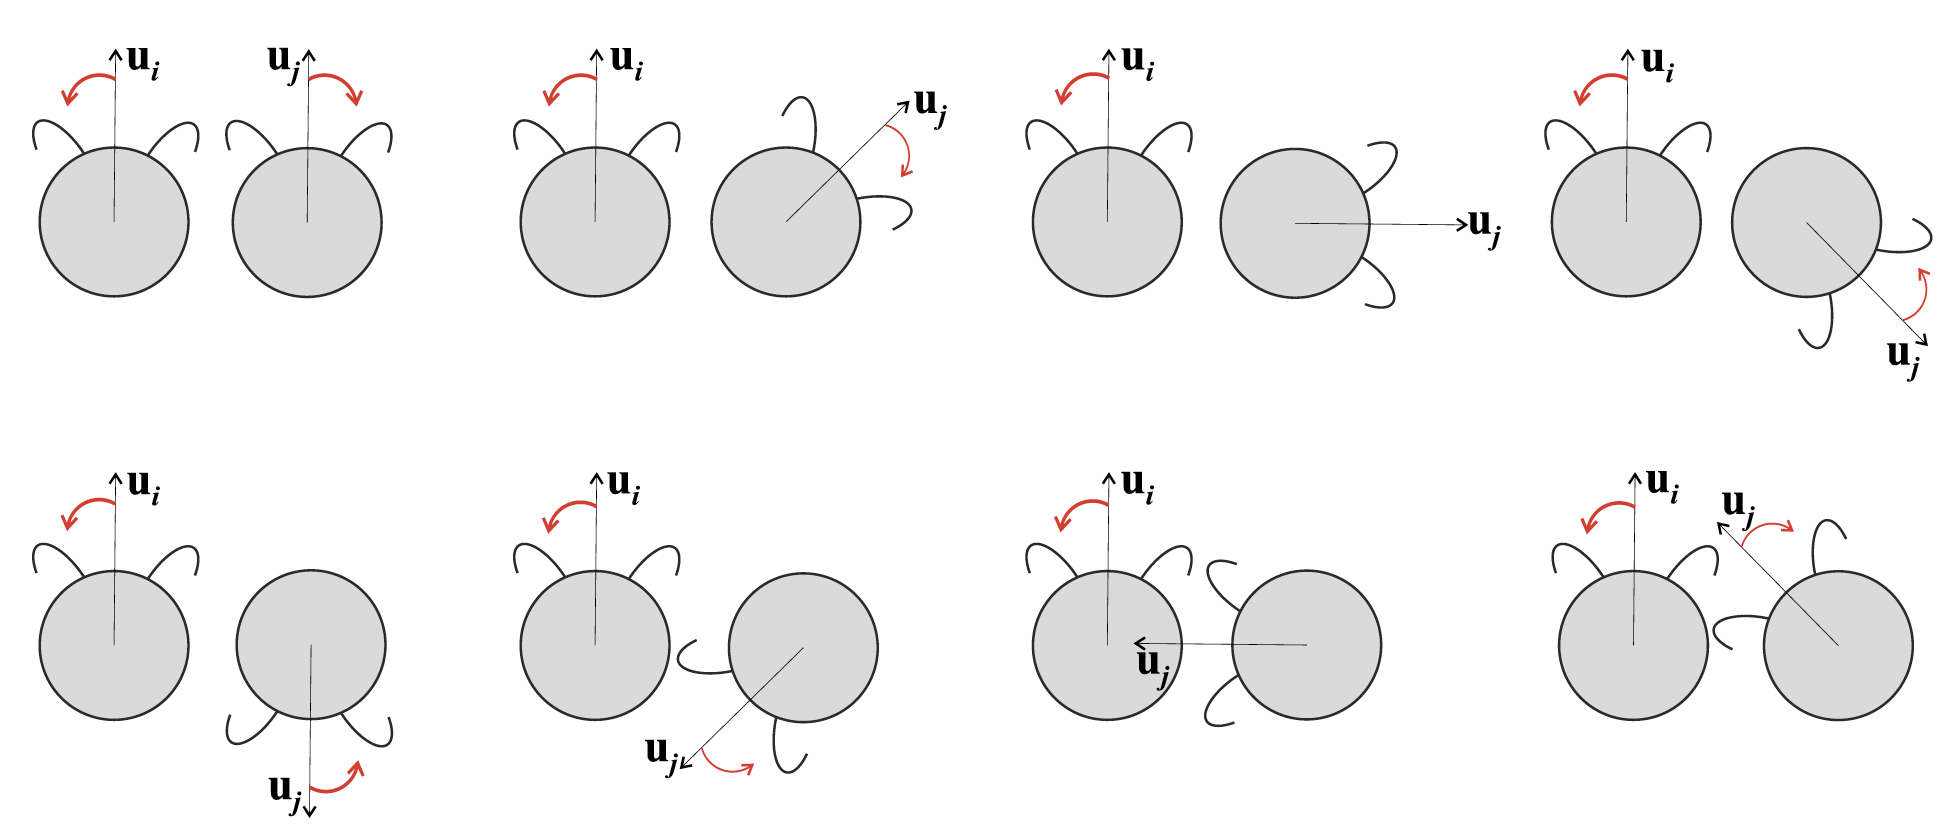
\includegraphics[width=1\textwidth]{Presentation/images/stark_behavior.png}\\
    A schematic of the encounter between two $Chlamydomonas$. 
    $u_i$ and $u_j$ the initial orientational vector and the rotation due to interaction shown in red.  
 \end{center}
 One can execute these simulations by running the command:
 \begin{verbatim}
    python Code/run.py sim_2_sq 2 filename
 \end{verbatim}
 The parameters can be changed in the \texttt{Code/run.py} and \\
 \texttt{Code/interactingsquirmers.py} files.\\
 We show the trajectories of the two squirmers as well as their initial orientation. The grey lines dotted
 represent the trajectories of the squirmers without any interaction, thus without any 
 force and torque applied on the squirmers. Circles are plotted at the start, 
 middle, and end of the simulation, with their radii proportional to the squirmers' size. The simulation is $T=0.8$
 with a time step $dt=1e^{-4}$.
 \begin{figure}[H]
    \centering
    \textbf{$\theta_2 = \frac{\pi}{2}$}\par\medskip
    \begin{minipage}{0.49\textwidth}
        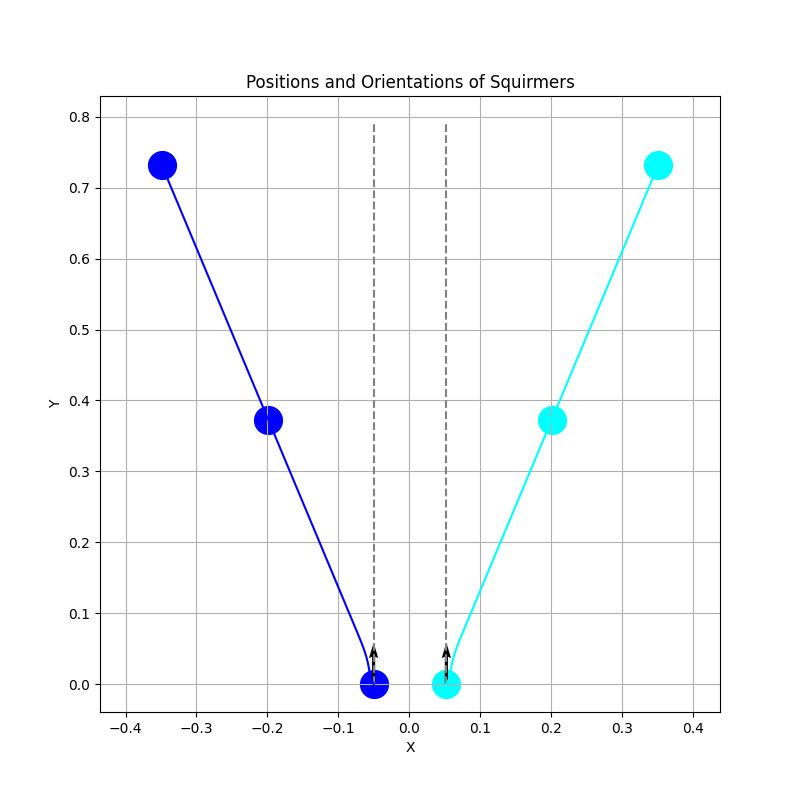
\includegraphics[width=1.1\textwidth]{graphs/simulations/sim_sq_sq/beta3/pi_2_.png}
        \caption{\footnotesize $\beta = 3$}
    \end{minipage}\hfill
    \begin{minipage}{0.49\textwidth}
        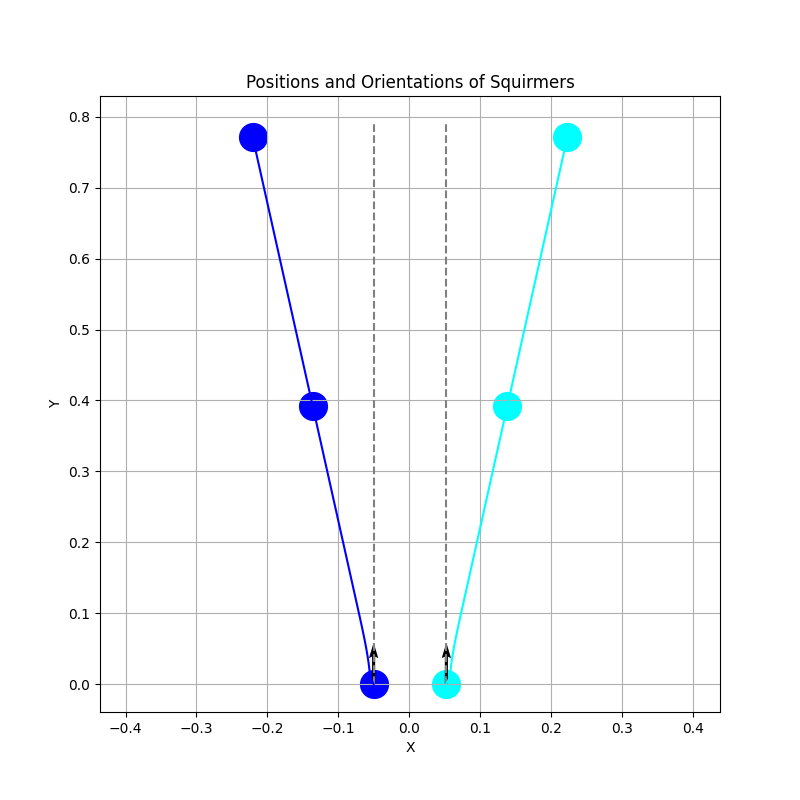
\includegraphics[width=1.1\textwidth]{graphs/simulations/sim_sq_sq/betam3/pi_2_.png}
        \caption{\footnotesize $\beta = -3$}
    \end{minipage}
\end{figure}
\begin{figure}[H]
    \centering
    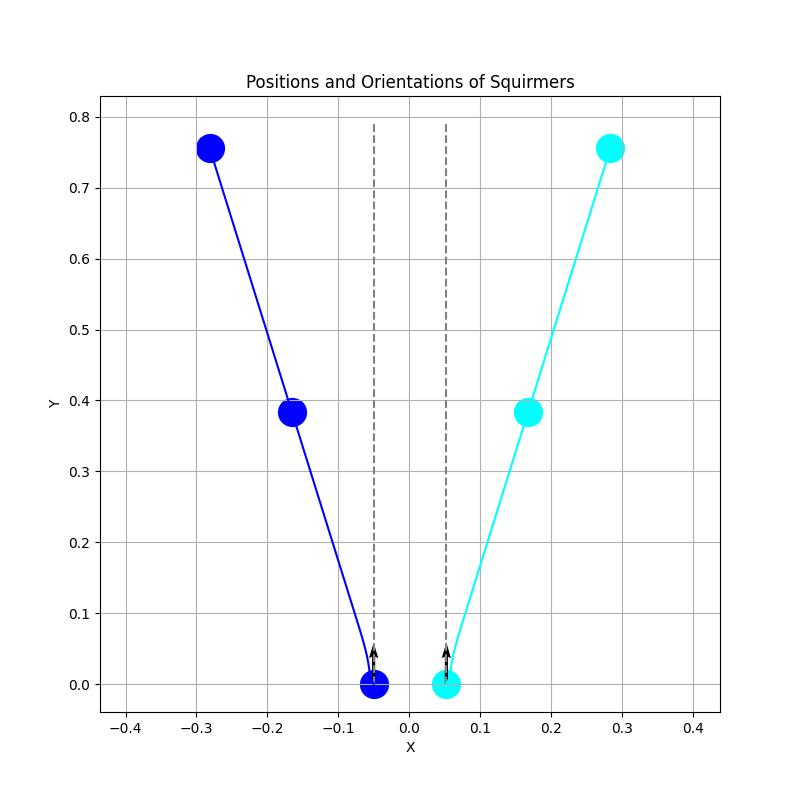
\includegraphics[width=0.55\textwidth]{graphs/simulations/sim_sq_sq/beta0/pi_2_.png}
    \caption{\footnotesize $\beta = 0$}
 \end{figure}
For $\theta_2 = \frac{\pi}{2}$, one can observe that their orientation changes due to the lubrification and steric forces which are applied on them. 
These forces and torques push the squirmers away from each other. and allow avoiding the overlapping of
 the two particles.\\
Each squirmer gradually distances itself from the other, consistent with the study \cite{Stark}.
For $\beta = 3$ the squirmers end the simulation at $x_1 = -0.35$ and $x_2 = 0.35$,
for $\beta = -3$ at $x_1 = -0.22$ and $x_2 = 0.22$,
 for $\beta = 0$ at $x_1 = -0.28$ and $x_2 = 0.28$.
 It is noteworthy that larger values of $\beta$ result in stronger forces and torques that push the
 squirmers further apart when both squirmers have an orientation $\theta = \frac{\pi}{2}$.
 \begin{figure}[H]
    \centering
    \textbf{$\theta_2 = \frac{3\pi}{4}$}\par\medskip
    \begin{minipage}{0.49\textwidth}
        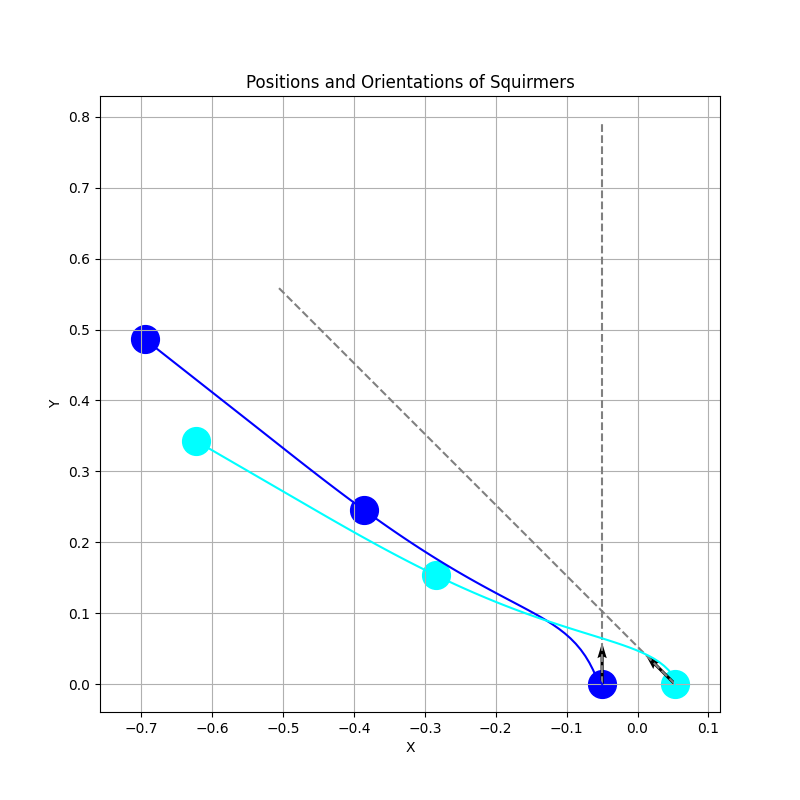
\includegraphics[width=1.1\textwidth]{graphs/simulations/sim_sq_sq/beta1_5/3pi_4_.png}
        \caption{\footnotesize $\beta = 1.5$}
    \end{minipage}\hfill
    \begin{minipage}{0.49\textwidth}
        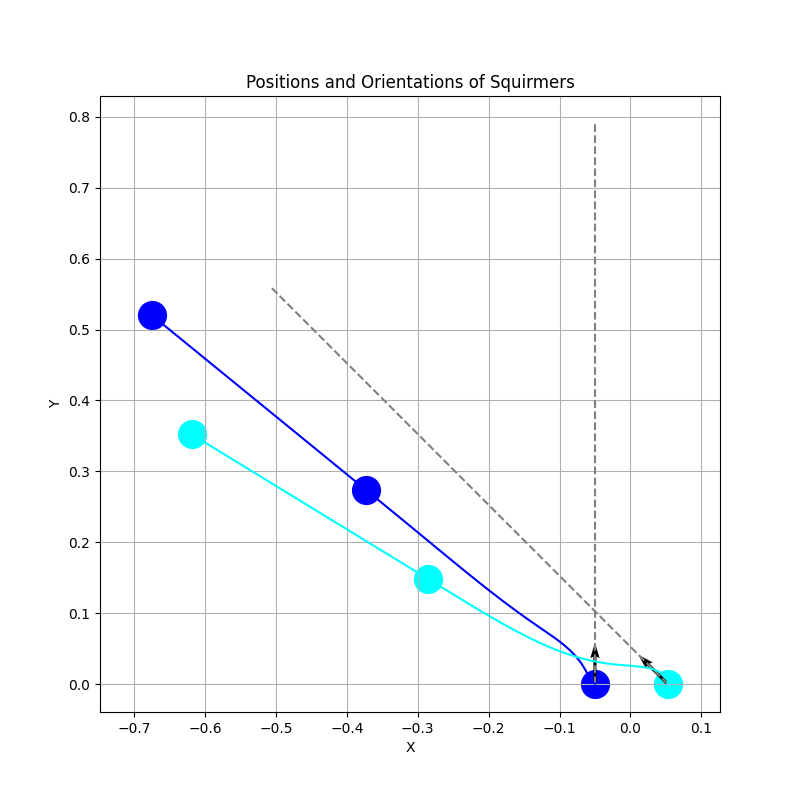
\includegraphics[width=1.1\textwidth]{graphs/simulations/sim_sq_sq/beta3/3pi_4_.png}
        \caption{\footnotesize $\beta = 3$}
    \end{minipage}
\end{figure}
\begin{figure}[H]
    \centering
    \begin{minipage}{0.49\textwidth}
        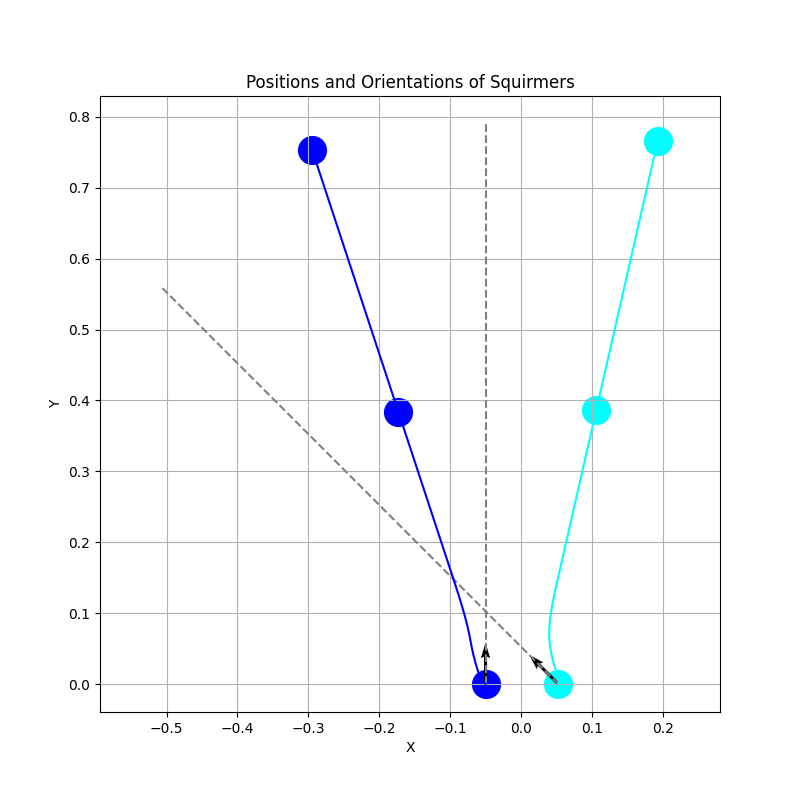
\includegraphics[width=1.1\textwidth]{graphs/simulations/sim_sq_sq/betam1_5/3pi_4_.png}
        \caption{\footnotesize $\beta = -1.5$}
    \end{minipage}\hfill
    \begin{minipage}{0.49\textwidth}
        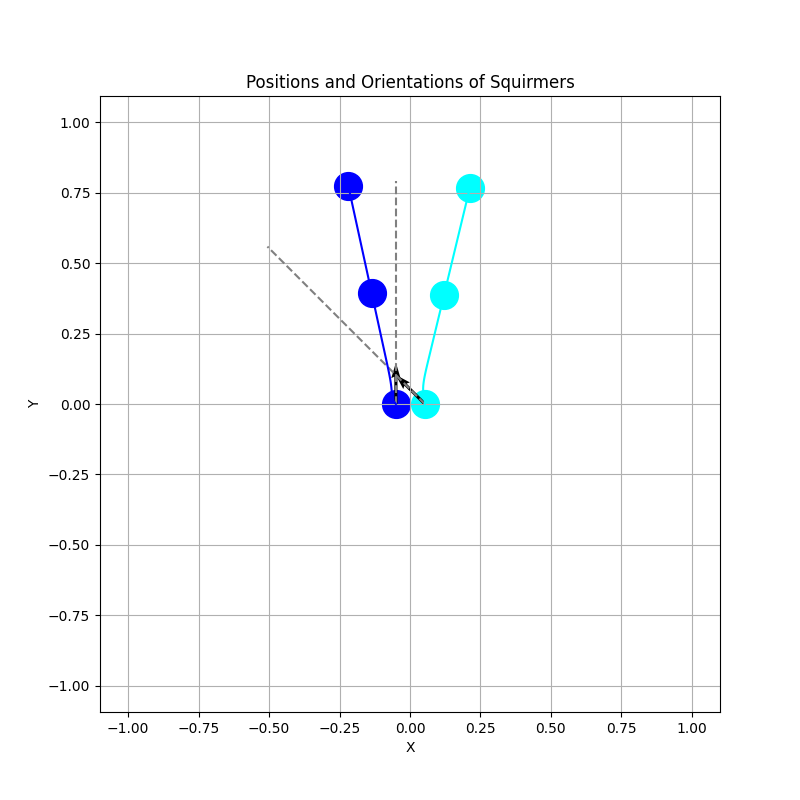
\includegraphics[width=1.1\textwidth]{graphs/simulations/sim_sq_sq/betam3/3pi_4_.png}
        \caption{\footnotesize $\beta = -3$}
    \end{minipage}
\end{figure}
\begin{figure}[H]
    \centering
    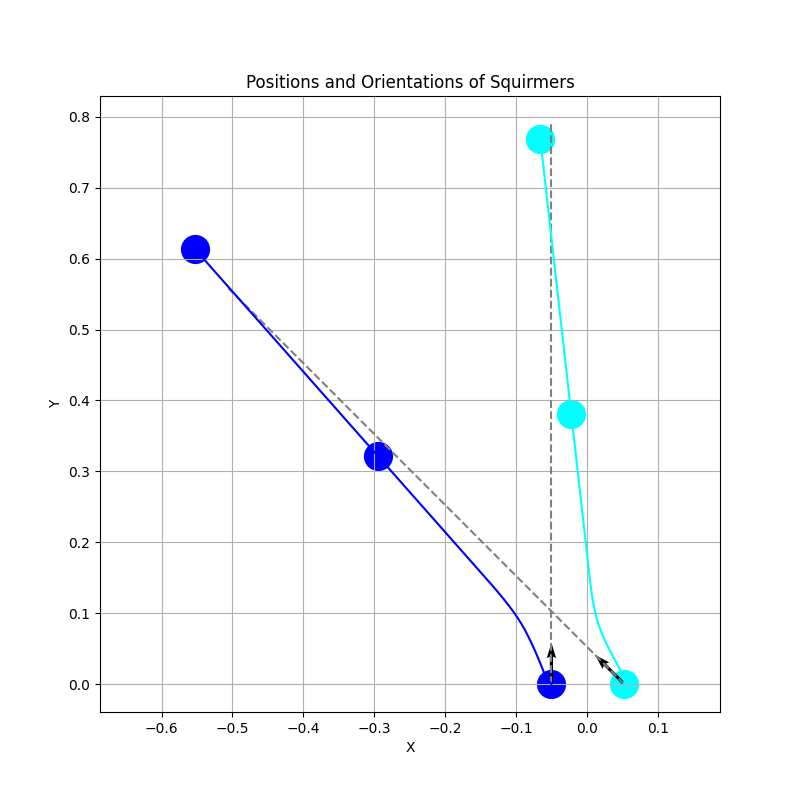
\includegraphics[width=0.55\textwidth]{graphs/simulations/sim_sq_sq/beta0/3pi_4_.png}
    \caption{\footnotesize $\beta = 0$}
\end{figure}
For the case $\theta_2 = \frac{3\pi}{4}$, ou results are consistent with the previous study\cite{Stark} for 
$\beta = 0$. However, for $\beta > 0$ the right 
squirmer is attracted to the left one,
 which does not correspond to the previous study. For $\beta < 0$ the torques on the right squirmer are larger than
 those acting on the left one, which also deviates from the previous study.\\
It is observed that for $\beta = 3$ the forces and torques pull the right squirmer towards the left one more strongly than for $\beta=1.5$.
Conversely, for $\beta = -3$ the right squirmer is pushed further away from the left one compared to $\beta = -1.5$.\\
In summary, for $\theta_2 = \frac{3\pi}{4}$, as $\beta$ increases, the right squirmer is more strongly pulled towards the left one. Conversely, as
$\beta$ decreases, the right squirmer is more strongly pushed away from the left one.


\begin{figure}[H]
    \centering
    \textbf{$\theta_2 = \pi$}\par\medskip
    \begin{minipage}{0.49\textwidth}
        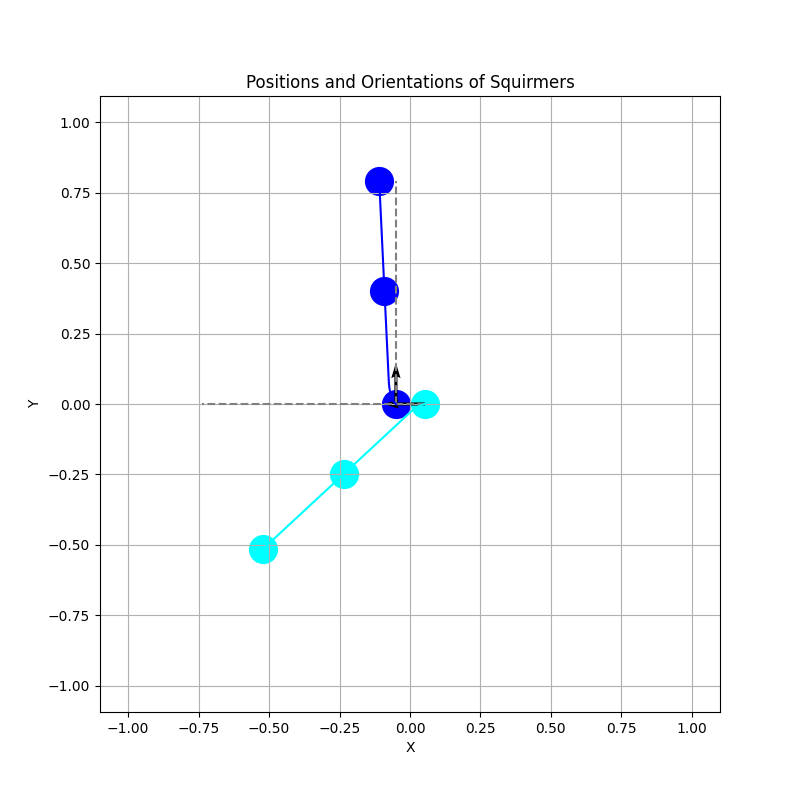
\includegraphics[width=1.1\textwidth]{graphs/simulations/sim_sq_sq/betam3/pi_.png}
        \caption{\footnotesize $\beta = -3$}
    \end{minipage}\hfill
    \begin{minipage}{0.49\textwidth}
        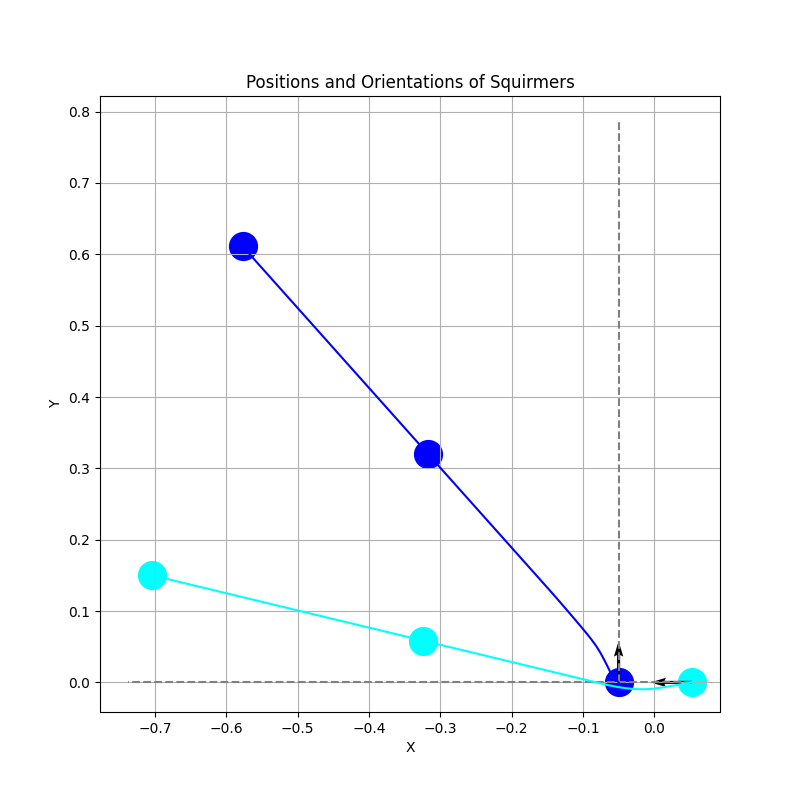
\includegraphics[width=1.1\textwidth]{graphs/simulations/sim_sq_sq/beta3/pi_.png}
        \caption{\footnotesize $\beta = 3$}
    \end{minipage}
\end{figure}
\begin{figure}[H]
    \centering
    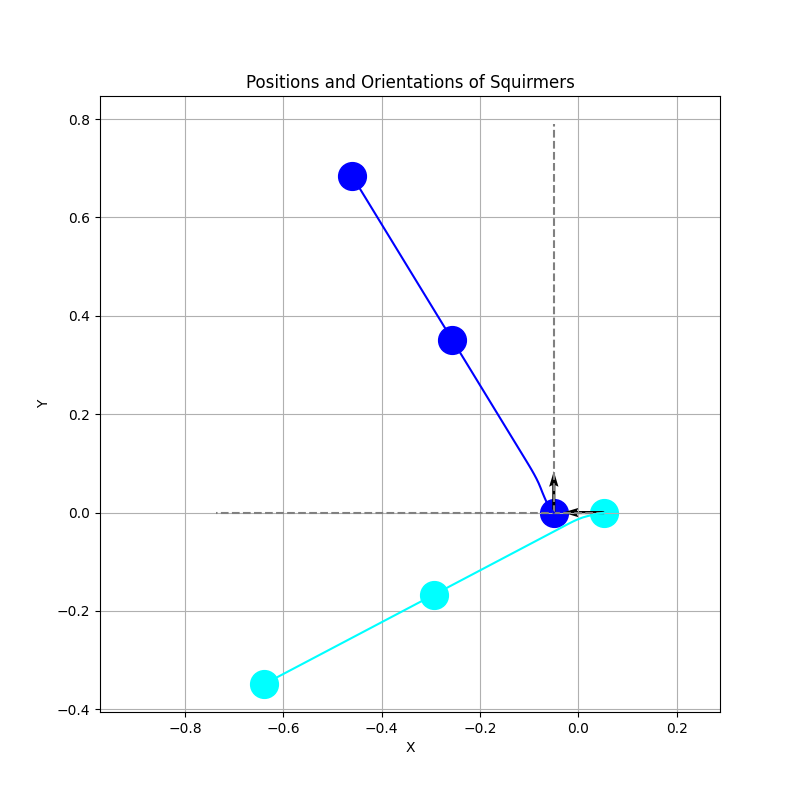
\includegraphics[width=0.55\textwidth]{graphs/simulations/sim_sq_sq/beta0/pi_.png}
    \caption{\footnotesize $\beta = 0$}
\end{figure}
For $\theta_2 = \pi$, these results are not consistent with the previous study\cite{Stark}. 
Our results show that the right squirmer's position
and orientation are altered by the forces and torques for any $\beta$ while the previous study showed that the right squirmer's
orientation is not supposed to change. Our results appear to be reasonable. The small initial 
distance between the squirmers, along with the applied forces and torques, causes the right 
squirmer to change its orientation.

\begin{figure}[H]
    \centering
    \begin{minipage}{0.49\textwidth}
        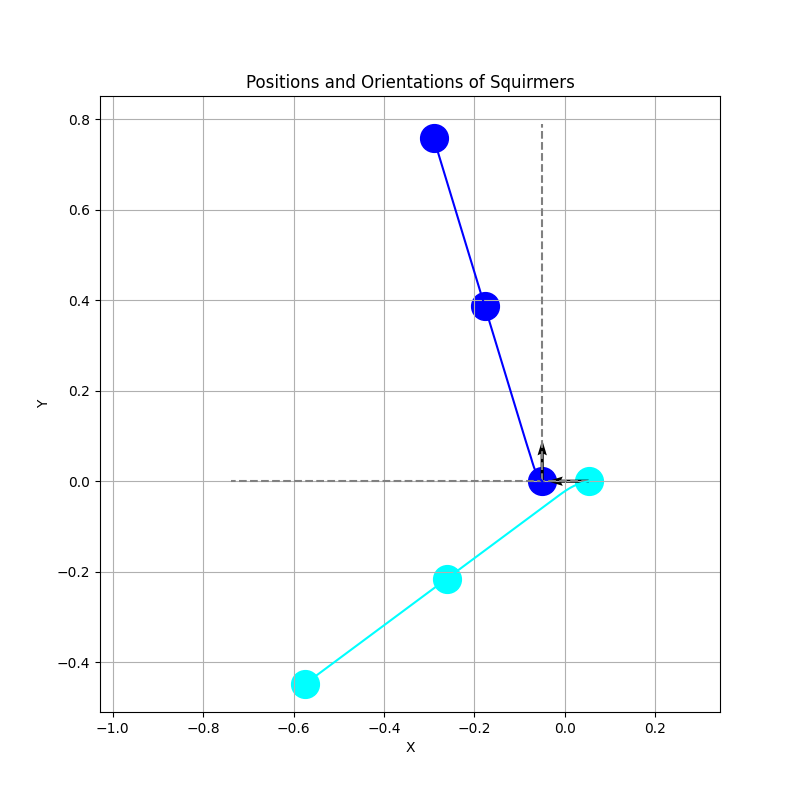
\includegraphics[width=1.1\textwidth]{graphs/simulations/sim_sq_sq/betam1_5/pi_.png}
        \caption{\footnotesize $\beta = -1.5$}
    \end{minipage}\hfill
    \begin{minipage}{0.49\textwidth}
        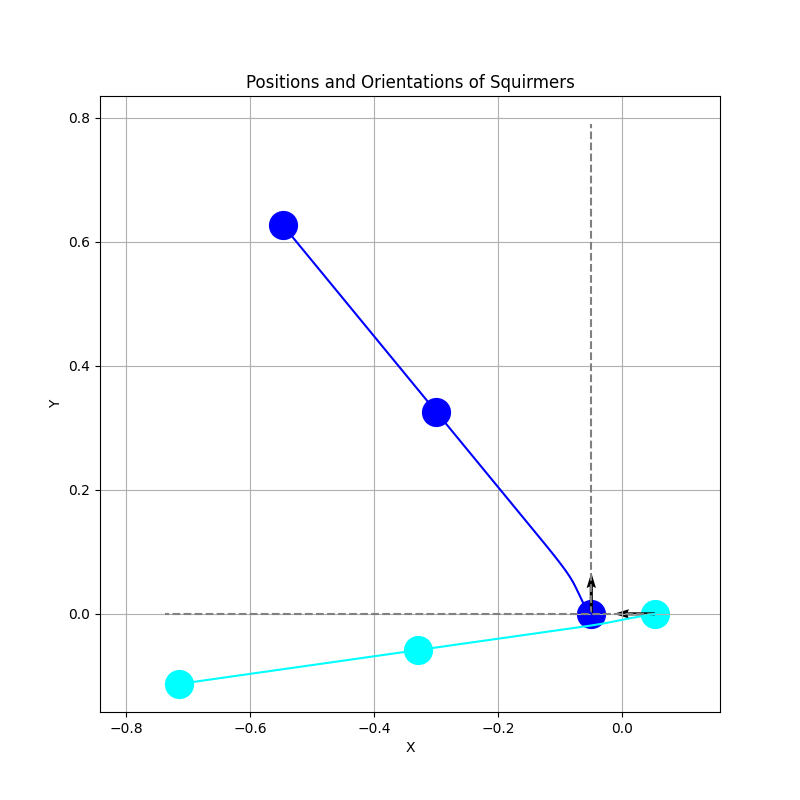
\includegraphics[width=1.1\textwidth]{graphs/simulations/sim_sq_sq/beta1_5/pi_.png}
        \caption{\footnotesize $\beta = 1.5$}
    \end{minipage}
\end{figure}
For $\beta = -3$, the orientation at the end of the simulation is less altered compared to $\beta = -1.5$.
For $\beta = 3$, the right squirmer ends up behind the left one, whereas for $\beta = 1.5$, the right
squirmer is pushed away.
These results indicate that for $\theta_2 = \pi$, as $\beta$ increases, the right squirmer is more strongly pulled 
towards the left one, while as $\beta$ decreases, the torques acting on the left squirmer also decrease.

\begin{figure}[H]
    \centering
    \textbf{$\theta_2 = -\frac{3\pi}{4}$}\par\medskip
    \begin{minipage}{0.49\textwidth}
        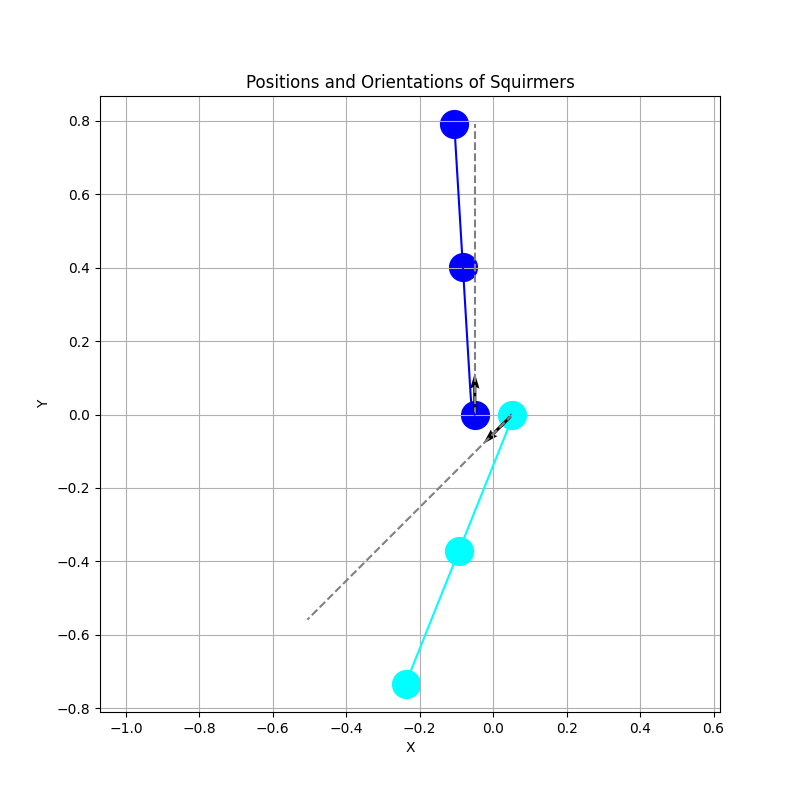
\includegraphics[width=1.1\textwidth]{graphs/simulations/sim_sq_sq/betam3/m3pi_4_.png}
        \caption{\footnotesize $\beta = -3$}
    \end{minipage}\hfill
    \begin{minipage}{0.49\textwidth}
        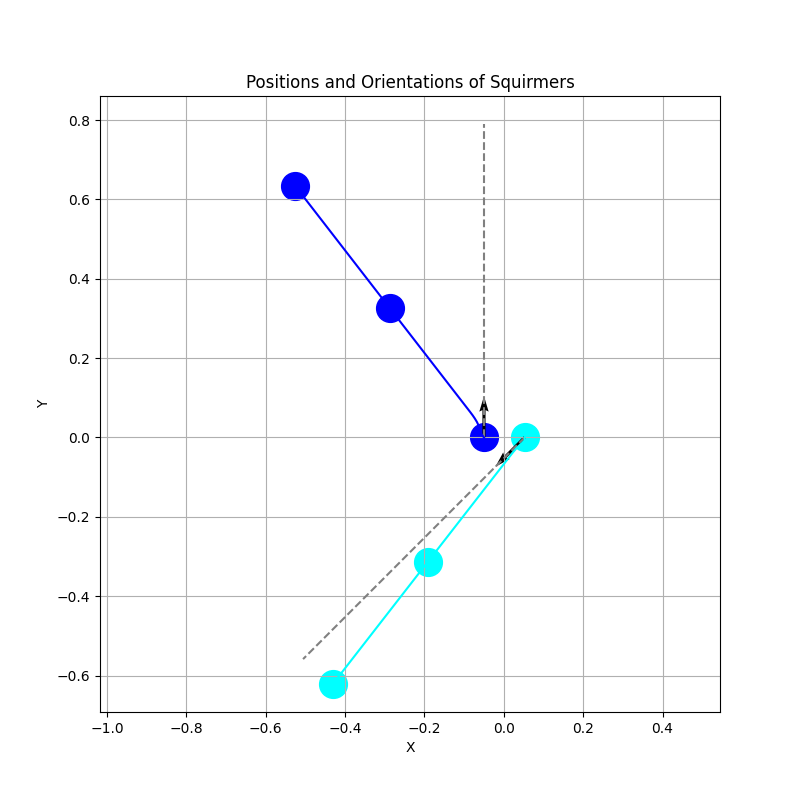
\includegraphics[width=1.1\textwidth]{graphs/simulations/sim_sq_sq/beta3/m3pi_4_.png}
        \caption{\footnotesize $\beta = 3$}
    \end{minipage}
\end{figure}
\begin{figure}[H]
    \centering
    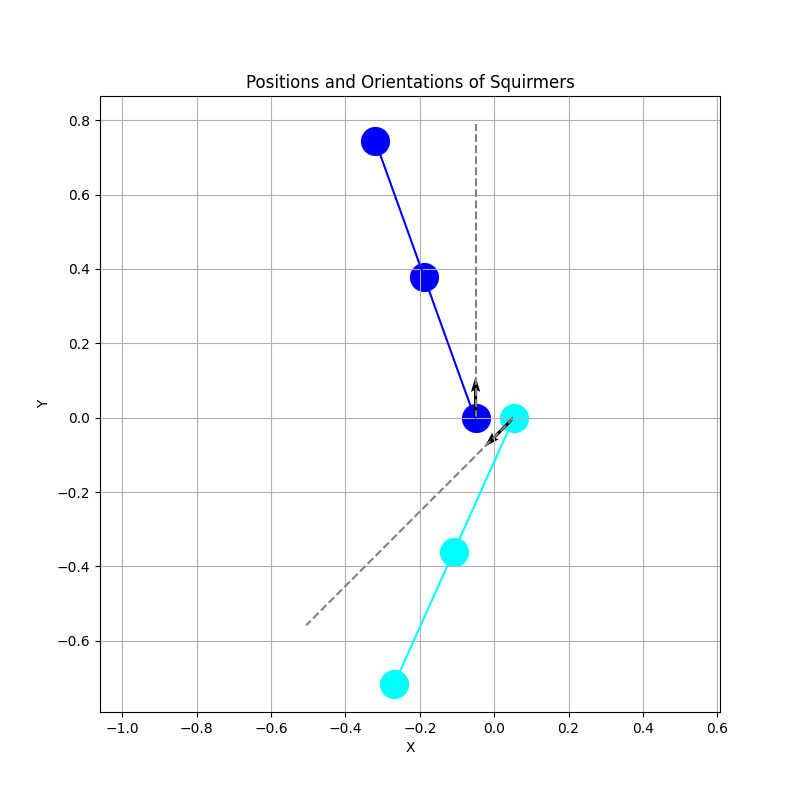
\includegraphics[width=0.55\textwidth]{graphs/simulations/sim_sq_sq/beta0/m3pi_4_.png}
    \caption{\footnotesize $\beta = 0$}
\end{figure}
For $\theta_2 = \frac{-3\pi}{4}$, these results are consistent with the previous study\cite{Stark} for $\beta \ge 0$ as the torques acting on the right squirmer
are weaker than the ones acting on the left one. On the contrary, for $\beta < 0$ the torques acting on the right squirmer are larger
than the ones acting on the left one.

\begin{figure}[H]
    \centering
    \textbf{$\theta_2 = -\frac{\pi}{2}$}\par\medskip
    \begin{minipage}{0.49\textwidth}
        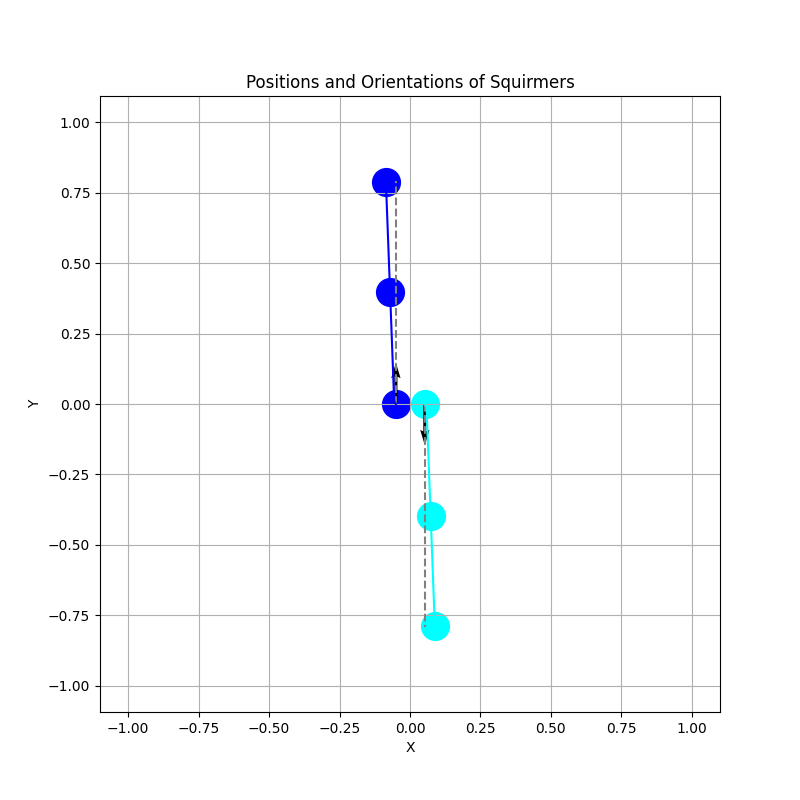
\includegraphics[width=1.1\textwidth]{graphs/simulations/sim_sq_sq/betam3/mpi_2_.png}
        \caption{\footnotesize $\beta = -3$}
    \end{minipage}\hfill
    \begin{minipage}{0.49\textwidth}
        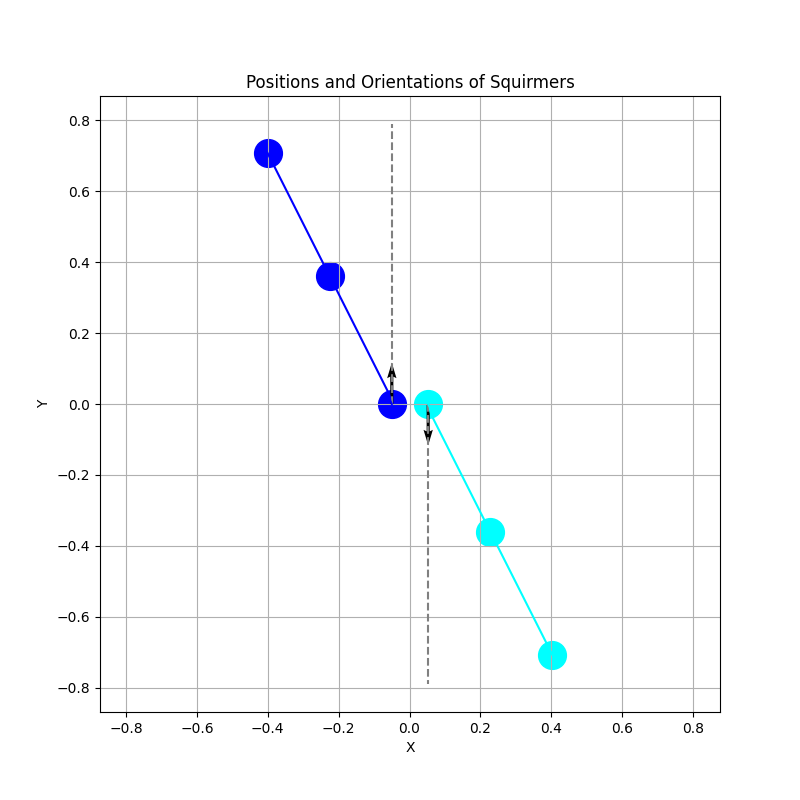
\includegraphics[width=1.1\textwidth]{graphs/simulations/sim_sq_sq/beta3/mpi_2_.png}
        \caption{\footnotesize $\beta = 3$}
    \end{minipage}
\end{figure}
\begin{figure}[H]
    \centering
    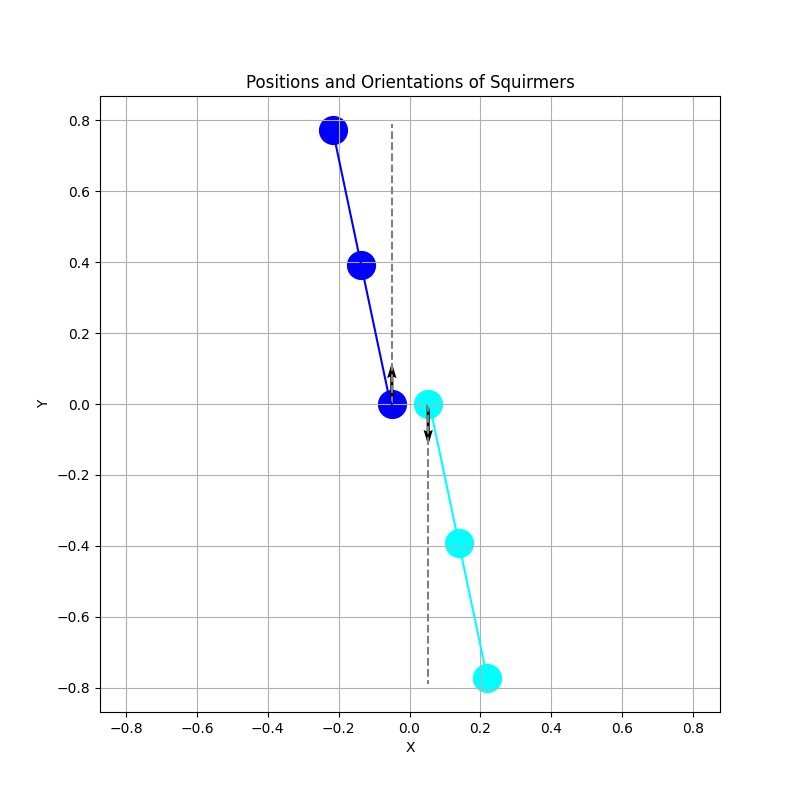
\includegraphics[width=0.55\textwidth]{graphs/simulations/sim_sq_sq/beta0/mpi_2_.png}
    \caption{\footnotesize $\beta = 0$}
\end{figure}
For $\theta_2 = \frac{-\pi}{2}$, our results are consistent with the previous study\cite{Stark} as the torques acting on the right squirmer are equal to
those acting on the left squirmer for all values of $\beta$.

\begin{figure}[H]
    \centering
    \textbf{$\theta_2 = -\frac{\pi}{4}$}\par\medskip
    \begin{minipage}{0.49\textwidth}
        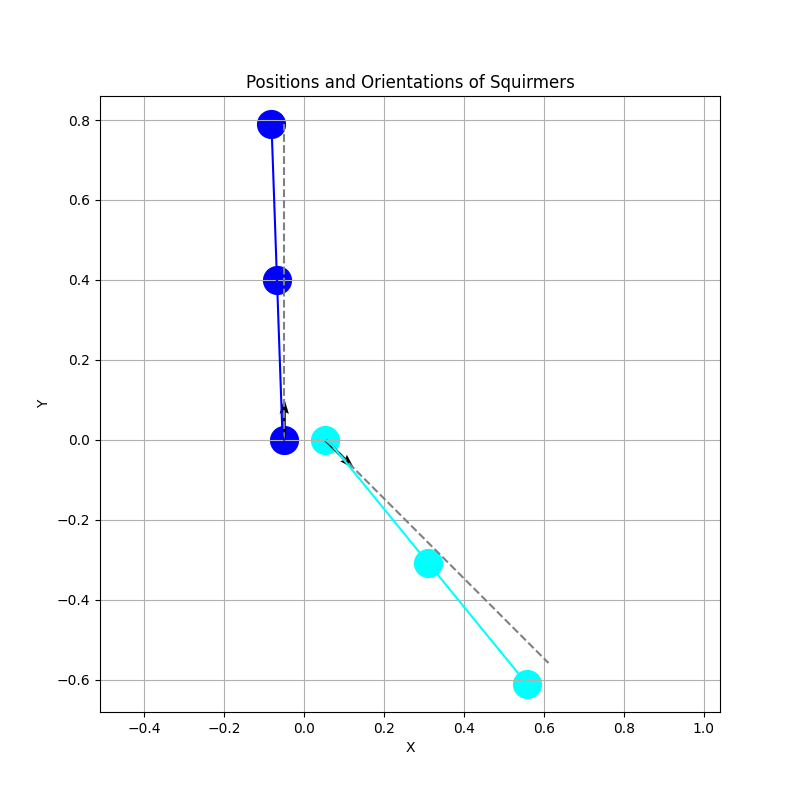
\includegraphics[width=1.1\textwidth]{graphs/simulations/sim_sq_sq/betam3/mpi_4_.png}
        \caption{\footnotesize $\beta = -3$}
    \end{minipage}\hfill
    \begin{minipage}{0.49\textwidth}
        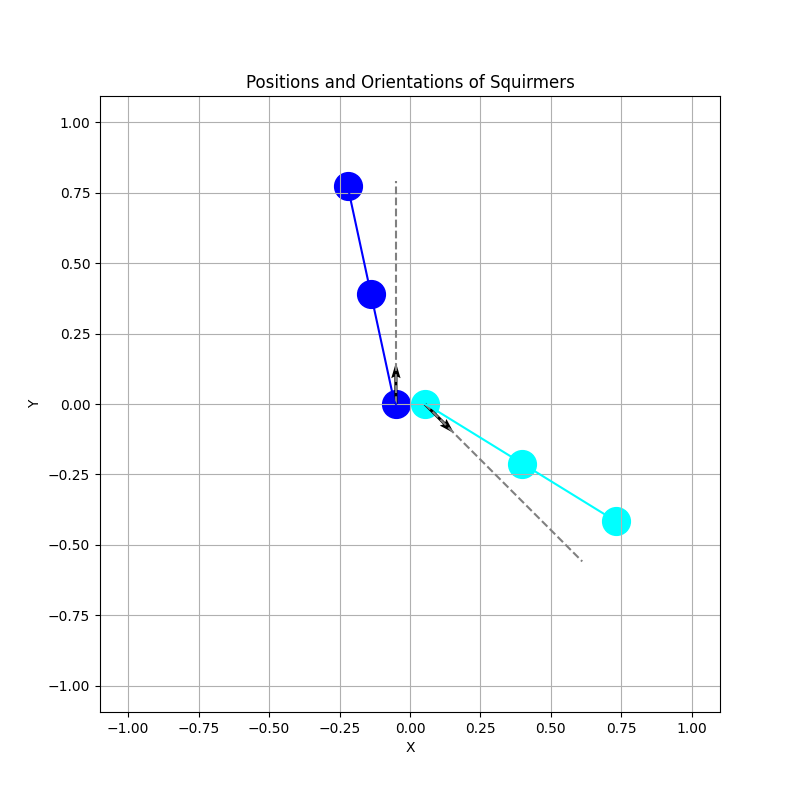
\includegraphics[width=1.1\textwidth]{graphs/simulations/sim_sq_sq/beta3/mpi_4_.png}
        \caption{\footnotesize $\beta = 3$}
    \end{minipage}
\end{figure}
\begin{figure}[H]
    \centering
    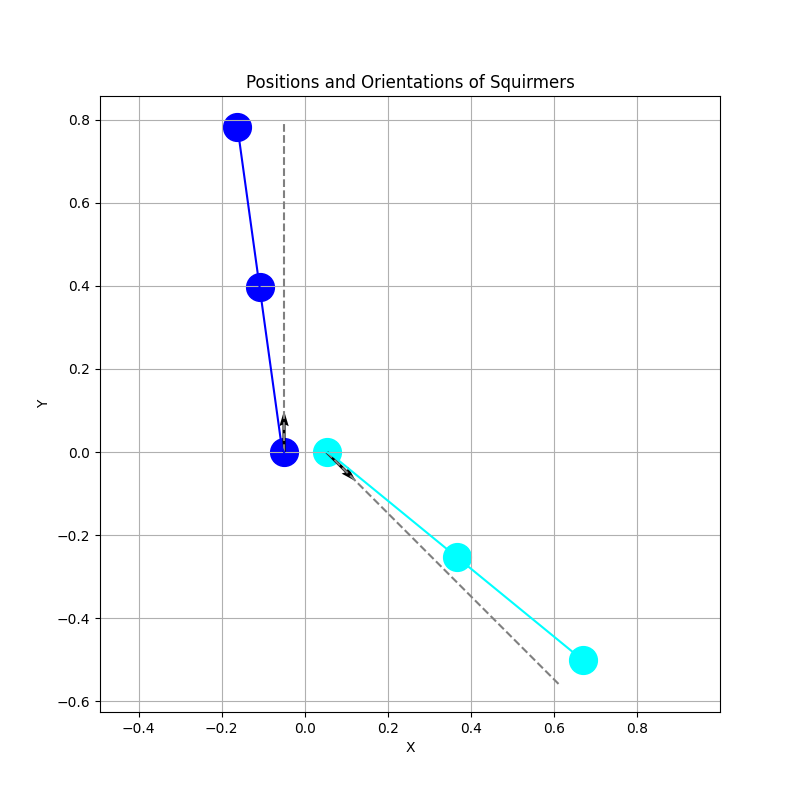
\includegraphics[width=0.55\textwidth]{graphs/simulations/sim_sq_sq/beta0/mpi_4_.png}
    \caption{\footnotesize $\beta = 0$}
\end{figure}
For case $\theta_2 = \frac{\pi}{4}$, these results are consistent with the previous study\cite{Stark} for $\beta = 0$ as the torques acting on the right 
squirmer are weaker to those acting on the left squirmer. For $\beta = 3$ the torques acting on the right squirmer are
equal to the those acting on the left squirmer which does not align with the previous study.
For $\beta = -3$ the direction of rotation does not align with the previous study.
\\
\\
\begin{figure}[H]
    \centering
    \textbf{$\theta_2 = \frac{\pi}{4}$}\par\medskip
    \begin{minipage}{0.49\textwidth}
        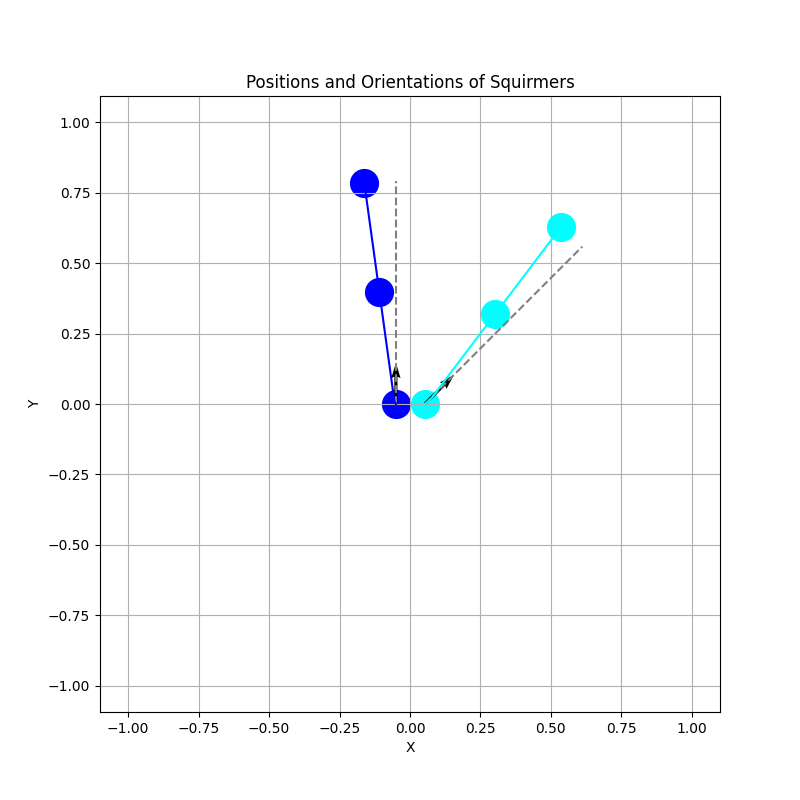
\includegraphics[width=1.1\textwidth]{graphs/simulations/sim_sq_sq/betam3/pi_4_.png}
        \caption{\footnotesize $\beta = -3$}
    \end{minipage}\hfill
    \begin{minipage}{0.49\textwidth}
        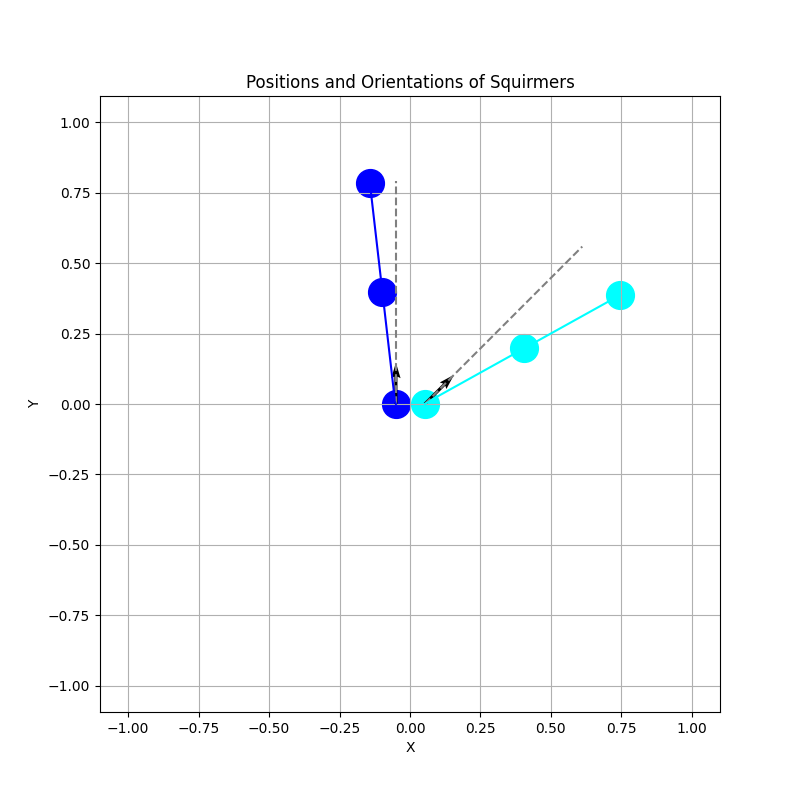
\includegraphics[width=1.1\textwidth]{graphs/simulations/sim_sq_sq/beta3/pi_4_.png}
        \caption{\footnotesize $\beta = 3$}
    \end{minipage}
\end{figure}
\begin{figure}[H]
    \centering
    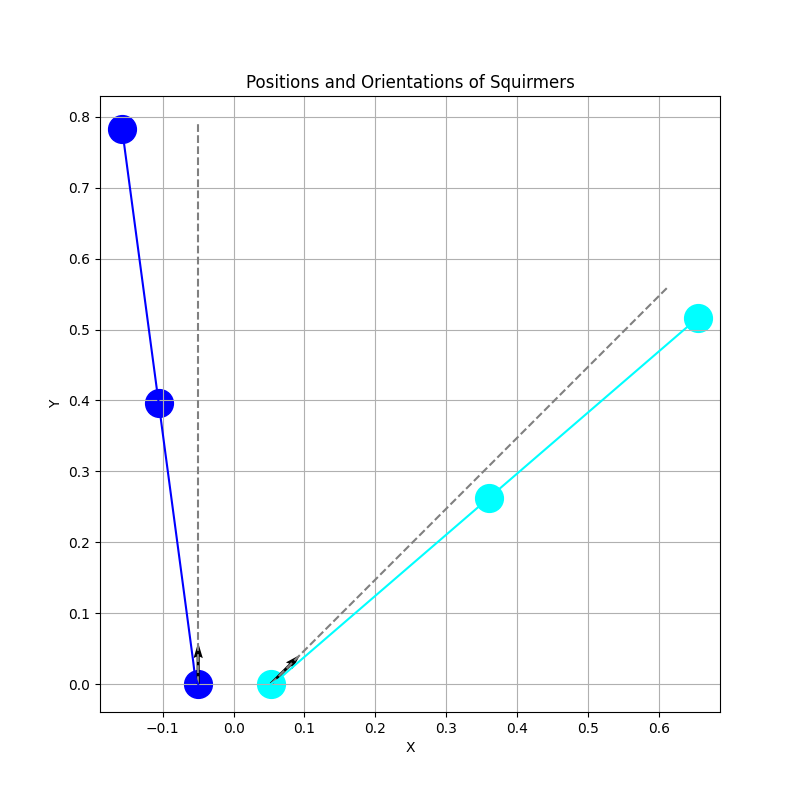
\includegraphics[width=0.55\textwidth]{graphs/simulations/sim_sq_sq/beta0/pi_4_.png}
    \caption{\footnotesize $\beta = 0$}
\end{figure}
For this last case, these results are consistent with the previous study\cite{Stark} for $\beta = 0$ as the torques acting on the right 
squirmer are weaker to those acting on the left squirmer. For $\beta = 3$ the torques acting on the right squirmer are
greater to the those acting on the left squirmer, which does not align with the previous study.
For $\beta = -3$ the direction of rotation does not align with the previous study.

\subsection{Simulation of squirmer-border interaction}
In this section simulations of a squirmer near a reflective border are conducted. The parameters of the simulations are fixed
except for the orientation and $\beta$ parameter. The squirmer is placed at $(x,y) = (-0.4,-0.7)$, has a radius of $R=0.05$,
a velocity $v_0=1$, a translational diffusivity $D=0$, an initial orientation $\theta$ varying among $-\frac{\pi}{6}$, $-\frac{\pi}{4}$, $-\frac{\pi}{3}$
and $-\frac{\pi}{2}$ and a $\beta$ value varying among $\beta_0 = 0, \beta_1 = 1.5, \beta_2 = 3, \beta_3 = -1.5, \beta_4 = -3$.
The border is placed at $y_b = -1$, the simulation time is $T = 0.9$ with a time step $dt = 1e^{-4}$.\\
One can execute these simulations by running the command:
 \begin{verbatim}
    python Code/run.py border 1 filename
 \end{verbatim}
 The parameters can be changed in the \texttt{Code/run.py} and \\
 \texttt{Code/interactingsquirmers.py} files.\\
 We show the trajectory of the squirmer as well as his initial orientation. A red circle and the corresponding time are marked when the squirmer
 reaches or exceeds the original height. Circles are plotted at the start, 
 middle, and end of the simulation, with their radii proportional to the squirmer's size.
 \begin{figure}[H]
    \centering
    \textbf{$\theta = -\frac{\pi}{6}$}\par\medskip
    \begin{minipage}{0.49\textwidth}
        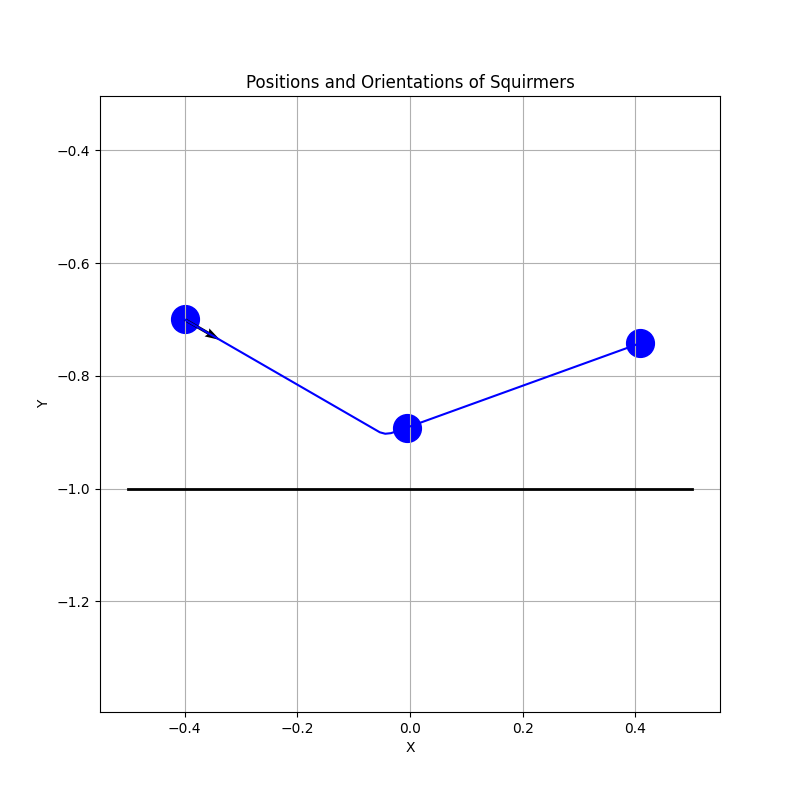
\includegraphics[width=1.1\textwidth]{graphs/simulations/border/beta1_5/mpi_6.png}
        \caption{\footnotesize $\beta = 1.5$}
    \end{minipage}\hfill
    \begin{minipage}{0.49\textwidth}
        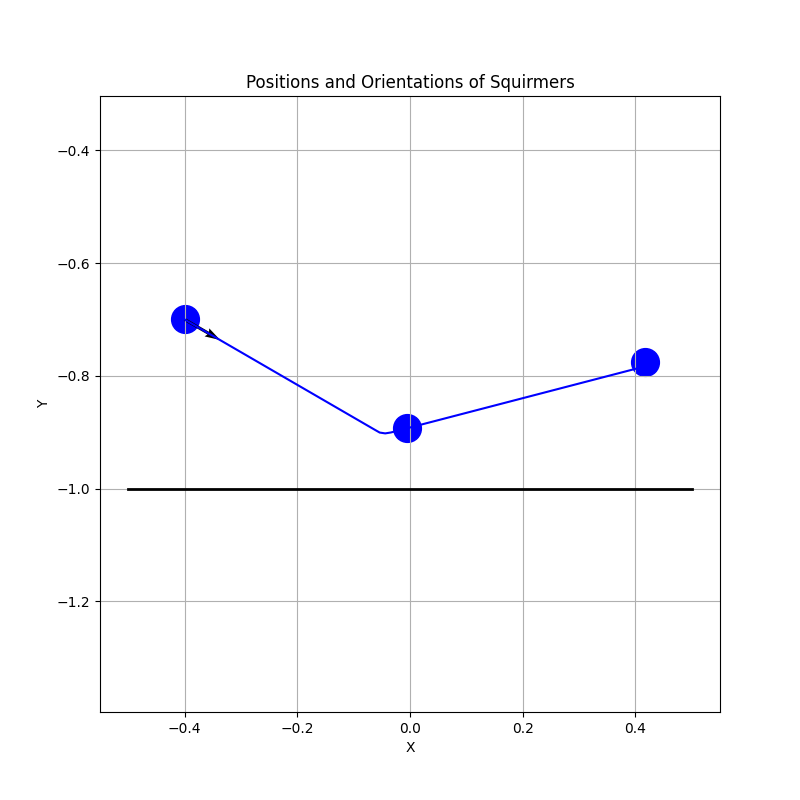
\includegraphics[width=1.1\textwidth]{graphs/simulations/border/beta3/mpi_6.png}
        \caption{\footnotesize $\beta = 3$}
    \end{minipage}
\end{figure}
\begin{figure}[H]
    \centering
    \begin{minipage}{0.49\textwidth}
        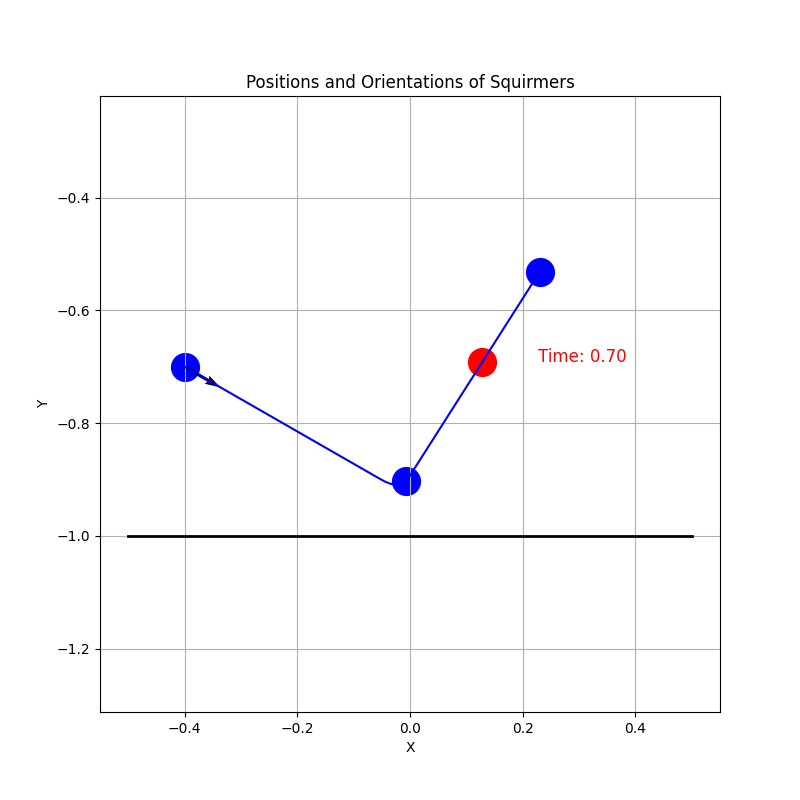
\includegraphics[width=1.1\textwidth]{graphs/simulations/border/betam1_5/mpi_6.png}
        \caption{\footnotesize $\beta = -1.5$}
    \end{minipage}\hfill
    \begin{minipage}{0.49\textwidth}
        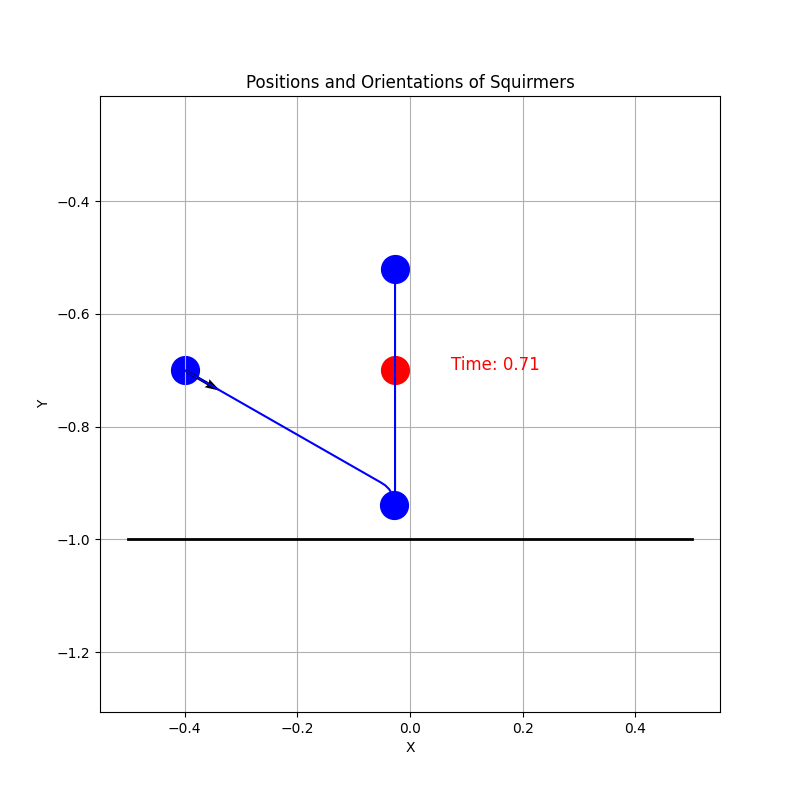
\includegraphics[width=1.1\textwidth]{graphs/simulations/border/betam3/mpi_6.png}
        \caption{\footnotesize $\beta = -3$}
    \end{minipage}
\end{figure}
\begin{figure}[H]
    \centering
    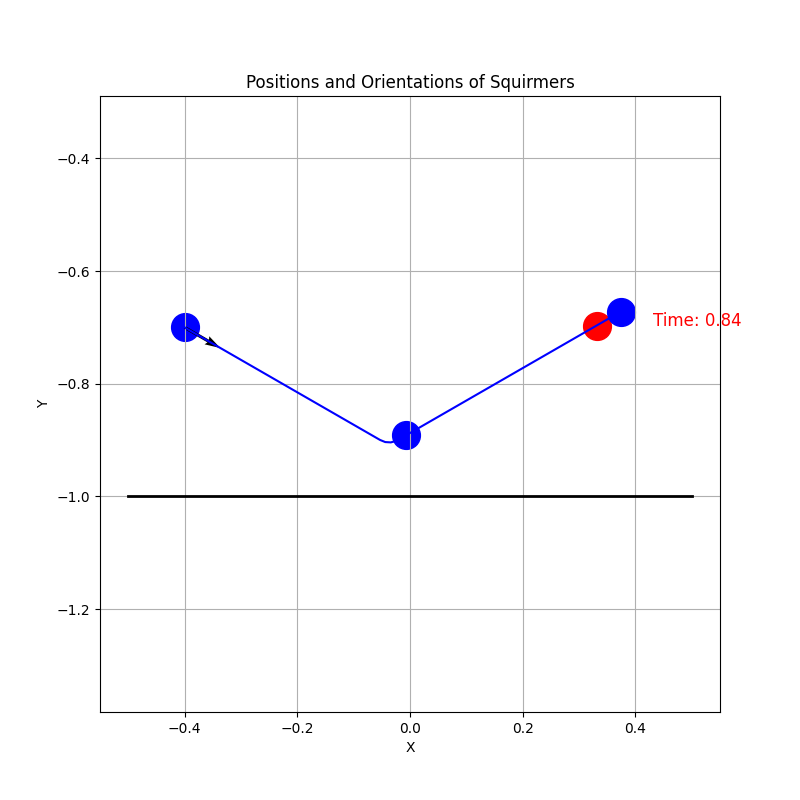
\includegraphics[width=0.55\textwidth]{graphs/simulations/border/beta0/mpi_6.png}
    \caption{\footnotesize $\beta = 0$}
\end{figure}
These results show that for $\theta = -\frac{\pi}{6}$, as $\beta$ increases, the squirmer's orientation upon interaction becomes parallel to the border.
On the contrary, as $\beta$ decreases, the squirmer's orientation upon interaction becomes tangential to the border.\\
The fact that the orientation after interaction is tangential does not necessarily mean that the particle reaches the initial 
height more quickly, as observed when $\beta = -3$ compared to when $\beta = -1.5$.

\begin{figure}[H]
    \centering
    \textbf{$\theta = -\frac{\pi}{4}$}\par\medskip
    \begin{minipage}{0.49\textwidth}
        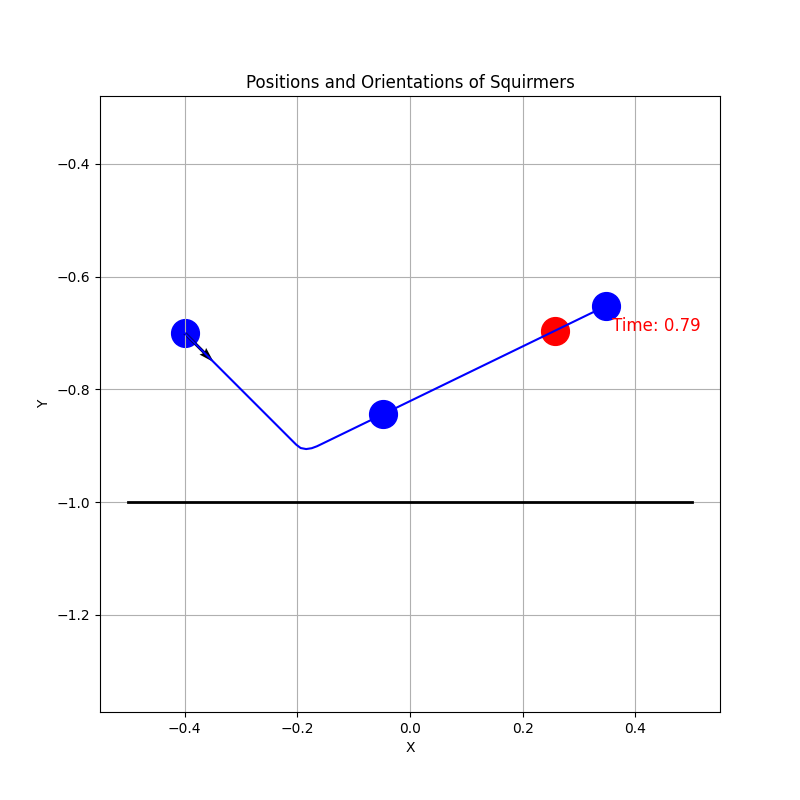
\includegraphics[width=1.1\textwidth]{graphs/simulations/border/beta1_5/mpi_4.png}
        \caption{\footnotesize $\beta = 1.5$}
    \end{minipage}\hfill
    \begin{minipage}{0.49\textwidth}
        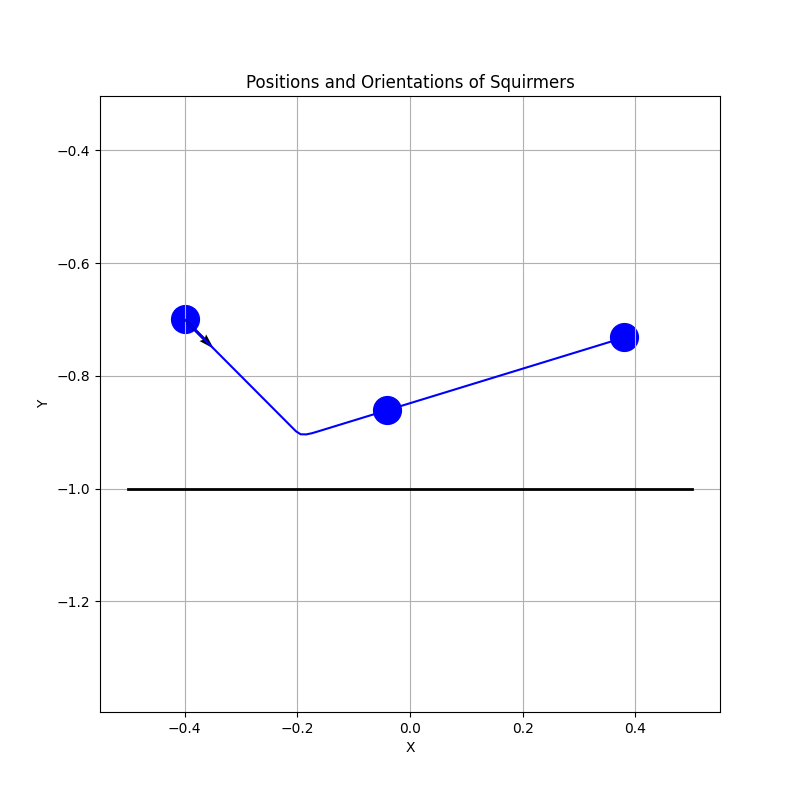
\includegraphics[width=1.1\textwidth]{graphs/simulations/border/beta3/mpi_4.png}
        \caption{\footnotesize $\beta = 3$}
    \end{minipage}
\end{figure}
\begin{figure}[H]
    \centering
    \begin{minipage}{0.49\textwidth}
        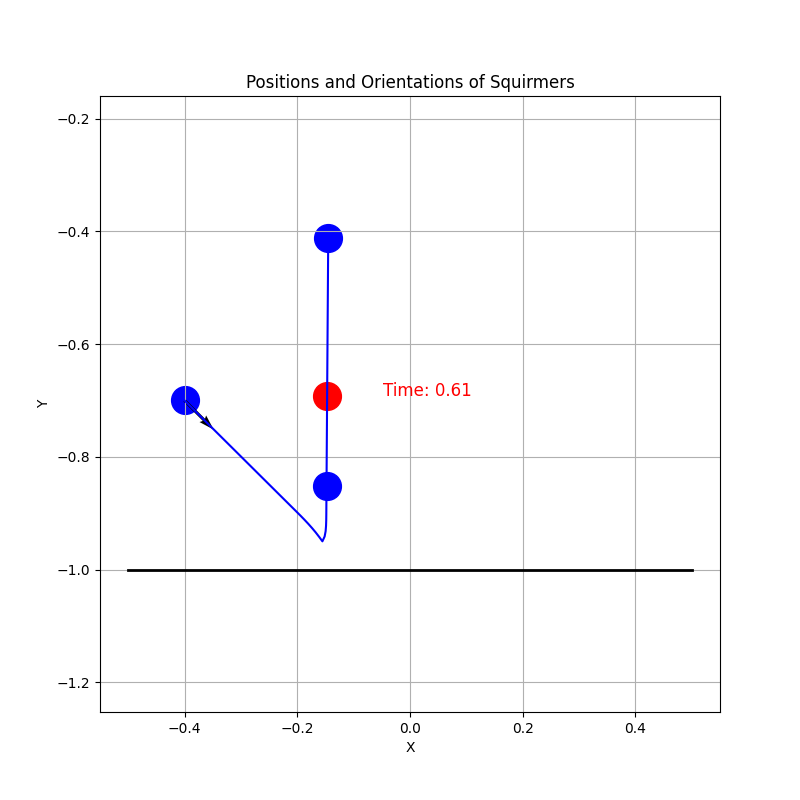
\includegraphics[width=1.1\textwidth]{graphs/simulations/border/betam1_5/mpi_4.png}
        \caption{\footnotesize $\beta = -1.5$}
    \end{minipage}\hfill
    \begin{minipage}{0.49\textwidth}
        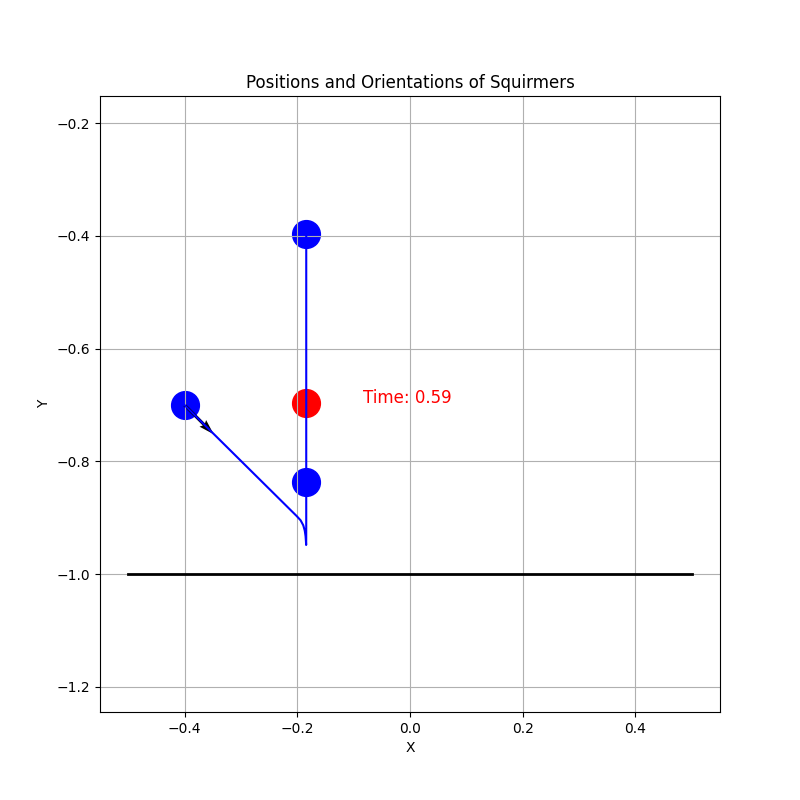
\includegraphics[width=1.1\textwidth]{graphs/simulations/border/betam3/mpi_4.png}
        \caption{\footnotesize $\beta = -3$}
    \end{minipage}
\end{figure}
\begin{figure}[H]
    \centering
    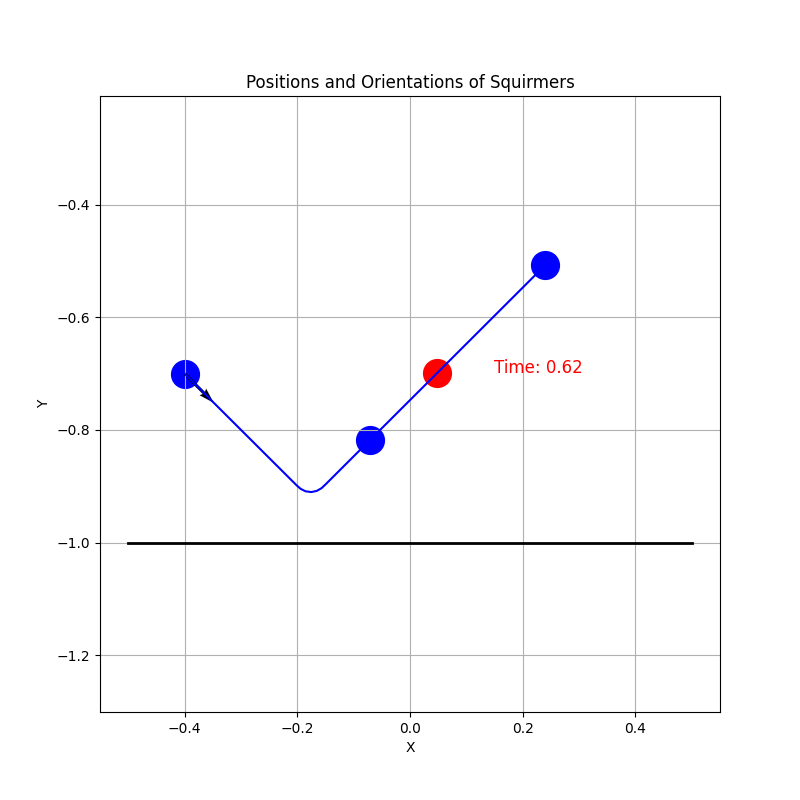
\includegraphics[width=0.55\textwidth]{graphs/simulations/border/beta0/mpi_4.png}
    \caption{\footnotesize $\beta = 0$}
\end{figure}
For $\theta = \frac{-\pi}{4}$ as well as for $\theta = \frac{-\pi}{3}$ and $\theta = \frac{-\pi}{2}$, 
the same observations are made, as $\beta$ increases (resp. decreases), the squirmer's 
orientation upon interaction becomes parallel (resp. tangential) to the border.\\
One can note that the initial orientation has an impact on the orientation after interaction with the border as for $\theta = -\frac{\pi}{4}$ and 
$\beta = 1.5$, the squirmer reaches and exceeds the original height during the simulation time. In contrast, for $\theta = -\frac{\pi}{6}$ and 
$\beta = 1.5$, the squirmer does not reach the initial height.

\subsection{$E_0$ parameter}
At the beginning of the internship, we studied the effect of the $E_0$ parameter on the alignment of the squirmers.\\
One can see the simulations and their resulting graphs in the \texttt{graphs/Eo\_analysis} and \texttt{videos/Eo\_analysis} directories.\\
The simulation is executed using:
\begin{verbatim}
    python3 Code/run.py Eo_sim 2 filename
\end{verbatim}
and one modify the \texttt{Code/run.py} file with the parameters one wants to test.
 Then for each $E_0$ given in \texttt{Code/run.py}, 
 a simulation is performed and the resulting graphs or videos are stored in the directories \texttt{graphs} or \texttt{videos}.\\

\subsubsection*{Evolution of the orientation}
First we used the expression given in reference:\cite{Lauga}.The torques acting on the squirmer $i$ can
 be calculated explicitly by:
$$
\Gamma_{i(j)\rightarrow i} = E_0p_i\hat{R}_{ij}^{\perp}(1 + \beta p_i\hat{R}_{ij})(ln \epsilon + O(1)),
$$
with $E_0$ the parameter to test and
$$
\Gamma_{j(i)\rightarrow i} = \frac{1}{4}\Gamma_{i(j)\rightarrow i}.
$$
We want to study the effect of $E_0$ on the alignment of squirmers in an open environment so $\Gamma_{i}^W$, which is the torque 
exerted by a wall on the squirmer vanishes.

\subsubsection*{Numerical Experiments}
The simulations are done with two squirmers placed at coordinates $(x_1, y_1) = (-R, 0)$ and $(x_2, y_2) = (\frac{2R}{1.5}, 0)$ with radius $R=0.05$, velocity $v_0=1$, viscosity $\mu = 1$, $\beta$ varying from $\beta_1 = 0$,
 $\beta_2 = -7.5$ and $\beta_3 = 7.5$, orientation $\theta_1 = \frac{\pi}{2}$ and $\theta_2$ varying between the major orientations of the unit circle.\\
 The values for the $E_0$ parameter are chosen from previous studies\cite{Brumley}\cite{Lauga}:
 $$
 E_{0_{1}} = \frac{3}{10}\frac{v_0}{R}, E_{0_{2}} = \frac{8}{5}\mu\pi a^2, E_{0_{3}} = \frac{-3}{2}\frac{v_0}{R},
 E_{0_{4}} = -E_{0_{1}}, E_{0_{5}} = -5$$
 $$
 E_{0_{6}} = \frac{5}{1000}, E_{0_{7}} = -2, E_{0_{8}} = -\frac{1}{2}, E_{0_{9}} = -E_{0_{8}}
 $$
We will show the results obtained for $\theta_2 = \pi$ and $\beta = 0$.
\begin{figure}[H]
    \centering
    \textbf{$\beta_1$ and $\theta_2 = \pi$}\par\medskip
    \begin{minipage}{0.49\textwidth}
        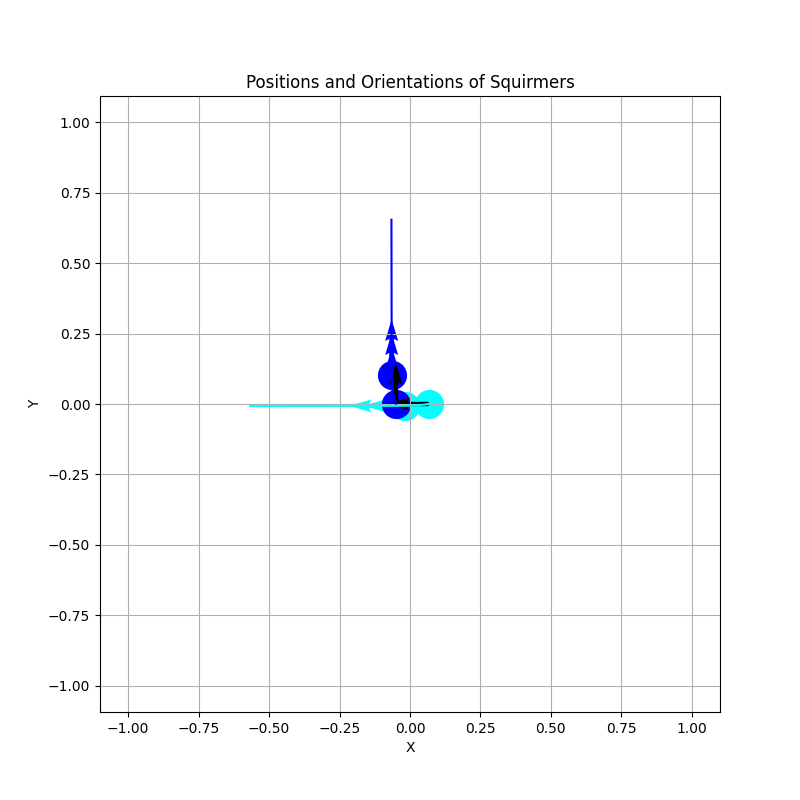
\includegraphics[width=1\textwidth]{graphs/Eo_analysis/beta0/pi_/pi_Eo_brumley.png}
        \caption{\footnotesize $E_{0_{2}}=\frac{8}{5}\mu\pi a^2$}
    \end{minipage}\hfill
    \begin{minipage}{0.49\textwidth}
        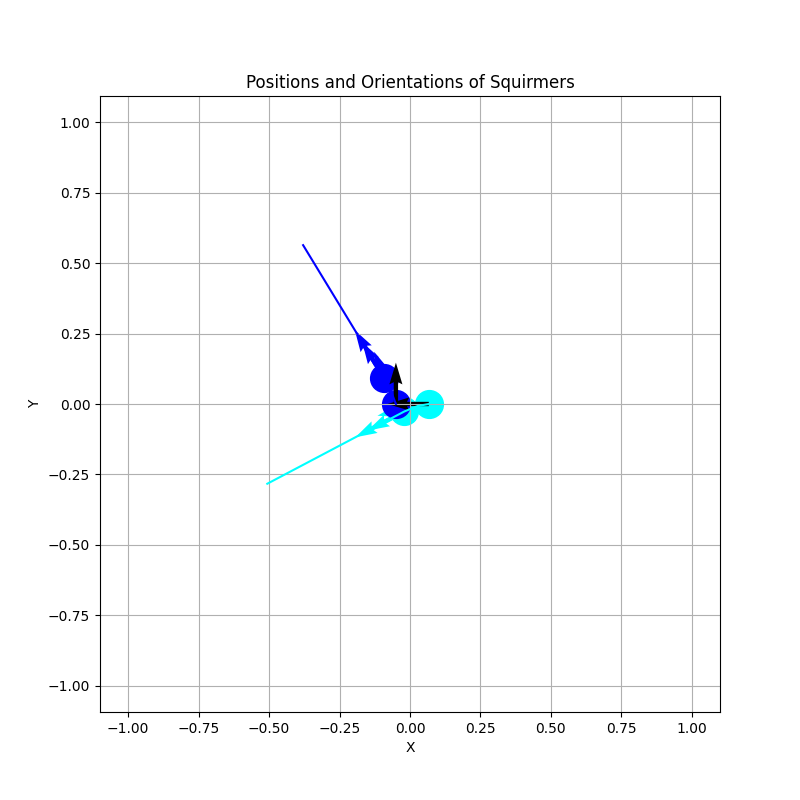
\includegraphics[width=1\textwidth]{graphs/Eo_analysis/beta0/pi_/pi_Eo_init.png}
        \caption{\footnotesize $E_{0_{1}}=\frac{3}{10}\frac{v_0}{R}$}
    \end{minipage}
\end{figure}
\begin{figure}[H]
    \centering
    \begin{minipage}{0.49\textwidth}
        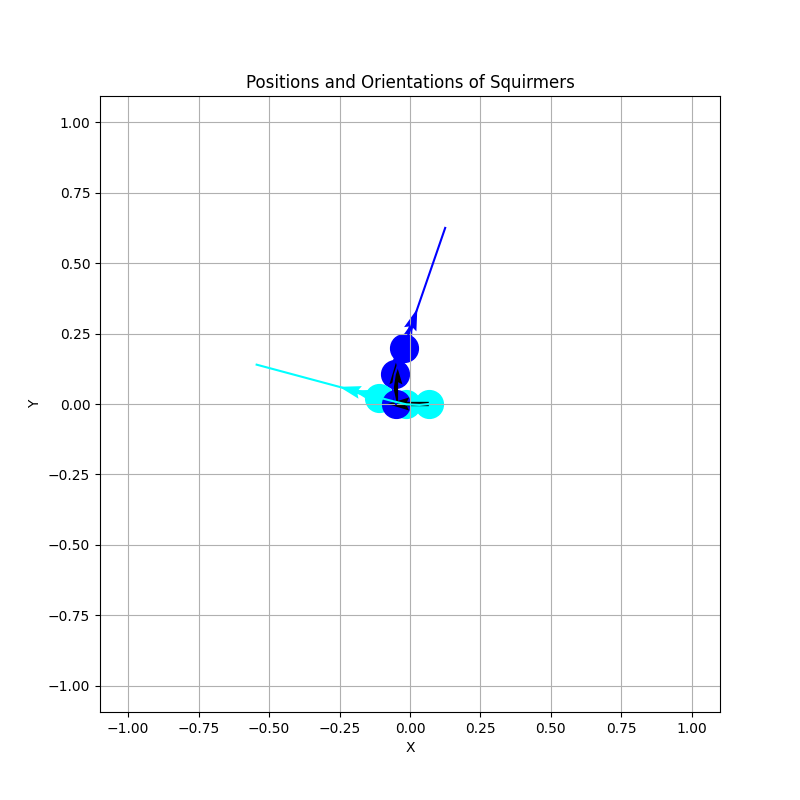
\includegraphics[width=1\textwidth]{graphs/Eo_analysis/beta0/pi_/pi_m2.png}
        \caption{\footnotesize $E_{0_{7}}=-2$}
    \end{minipage}\hfill
    \begin{minipage}{0.49\textwidth}
        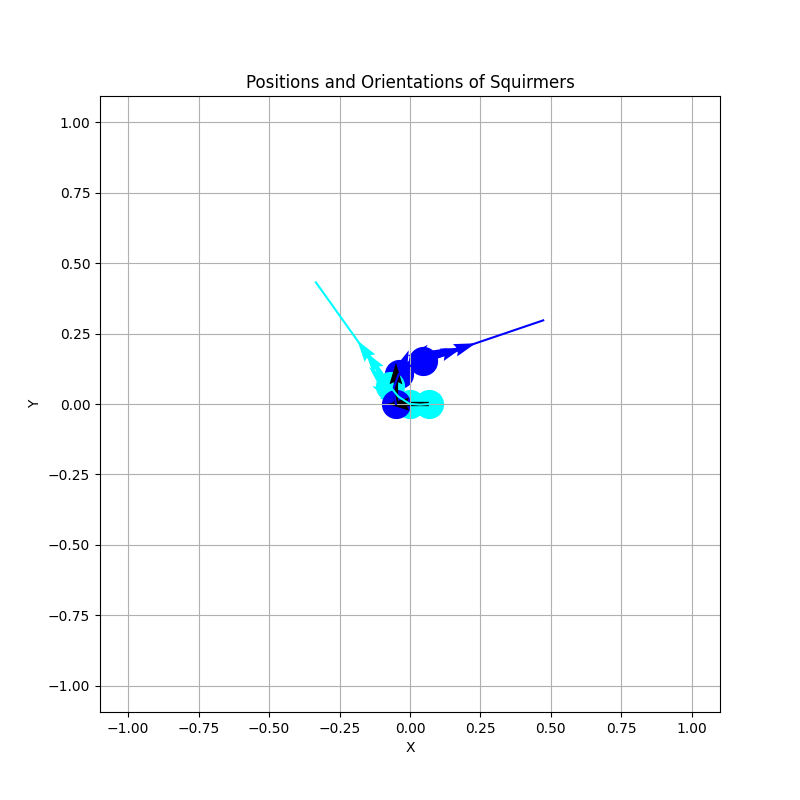
\includegraphics[width=1\textwidth]{graphs/Eo_analysis/beta0/pi_/pi_m5.png}
        \caption{\footnotesize $E_{0_{5}}=-5$}
    \end{minipage}
    The arrows show the changes of orientations and a circle is plotted every four times the orientation of a squirmer is affected.
\end{figure}
Our results show that as $E_0$ decreases, the torques acting on the squirmers become stronger, as 
demonstrated by the example of $E_0 = -5$. 
No value of $E_0$
could be found that allows the alignment of the squirmers. The alignment of the particles 
could not be controlled by varying the parameter $E_0$. The same conclusion was reached for all other tested values of $\beta$
and $\theta$.

\subsection{Simulation of N squirmers}
In this section, simulations of $375$ squirmers are conducted in a rectangle with dimensions $L_y = 3$ and $L_x=6$, over 
a simulation time of $T=10$. Two types of boundary conditions are considered: a box with reflective boundaries, 
and a channel with reflective boundaries in the y-direction and periodic boundaries in the x-direction.
The squirmers have a radius of $R = 0.02$, a velocity of $v_0 = 1$, a translational diffusivity of $D=0$, and $\beta = 0$.
 They are randomly positioned within the rectangle, each with a random orientation. The minimum distance between 
 squirmers, as well as the polar order parameter, are plotted at the end of each simulation.\\
One can do a simulation by running:
\begin{verbatim}
    python Code/run.py video N filename
\end{verbatim} 
where \texttt{N} is the number of squirmers, and \texttt{filename} is the name of the output file.
\begin{figure}
    \begin{minipage}{0.49\textwidth}
        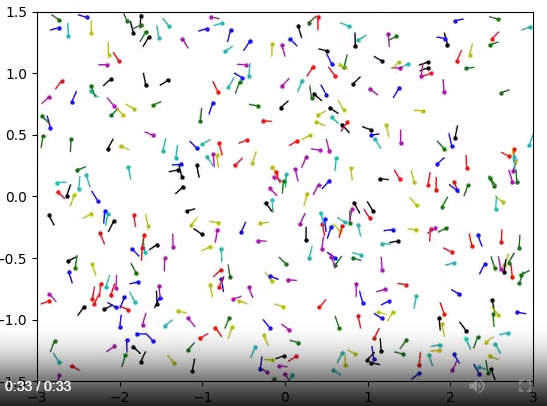
\includegraphics[width=1\textwidth]{Presentation/images/simulation.png}
        \caption{Simulation of squirmers within a box}
    \end{minipage}\hfill
    \begin{minipage}{0.49\textwidth}
        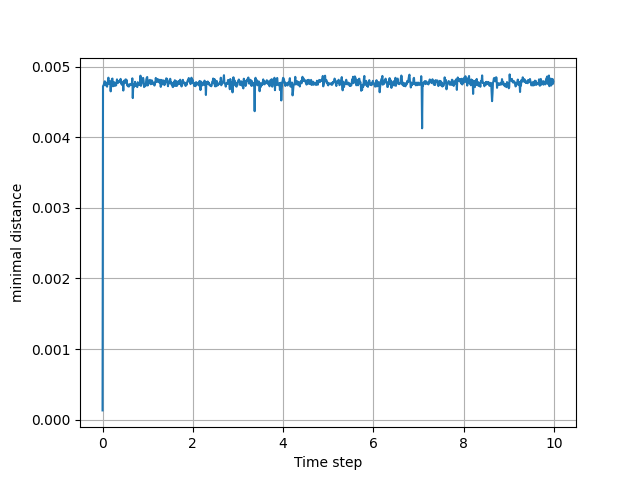
\includegraphics[width=1\textwidth]{videos/min_dist_box2.png}
        \caption{\footnotesize Minimum distance between squirmers over time}
    \end{minipage}
\end{figure}
The squirmers are represented with their orientations and one can see the videos in the \texttt{videos} directory. The minimal
distance and polar order parameter, defined in the following section, are also plotted. 
Note that in the channel configuration, the minimum distance can appear negative due to the periodic boundaries, 
which can position one squirmer on top of another.

\subsection{Study of $D$ parameter}
In this section, simulations are conducted with $375$ squirmers in a channel, with a simulation time of $T=50$ and a time step of $dt=1e^{-4}$. 
The squirmers have 
a radius of $R = 0.02$, a velocity of $v_0 = 1$, a range of $\beta$ values:
$\beta_0 = 0, \beta_1 = 1.5, \beta_2 = 3, \beta_3 = -1.5, \beta_4 = -3$
 and a translational diffusivity varying among:
$$D_0 = 0.5, D_1 = 1, D_2 = 3.$$
Two different sizes of channel are used: $Ch_1$ with dimensions $L_y = 3$ and $L_x = 6$ and $Ch_2$ with dimensions $L_y=2$ and $L_x=4$. 
The objective is to examine 
the impact on the particle density $\rho$ on collective behavior, $\rho$ is given by:
$$\rho = \frac{N\pi R^2}{L_xL_y}.$$
The squirmers are randomly positioned within the channel, each with a random orientation.
For simulations with the same $\beta$ and $\rho$, the initial positions and orientations of the squirmers are identical,
ensuring that the only varying parameter between two simulations is the diffusivity $D$.\\
To analyze the collective behavior of the squirmers, the polar order parameter $v_a$ is employed:
$$v_a = \frac{1}{N}\left|\sum^{N}_{i=1}p_i\right|,$$
where $p_i$ denotes the orientation of the $i$-th squirmer.
A value of $v_a = 1$ indicates that all squirmers are moving in the same direction, while $v_a\approx 0$ suggests uncorrelated motions.
\begin{figure}[H]
    \centering
    \textbf{$Ch_1$($L_x = 6$ and $L_y = 4$), $\rho = 0.026$}\par\medskip
    \begin{minipage}{0.49\textwidth}
        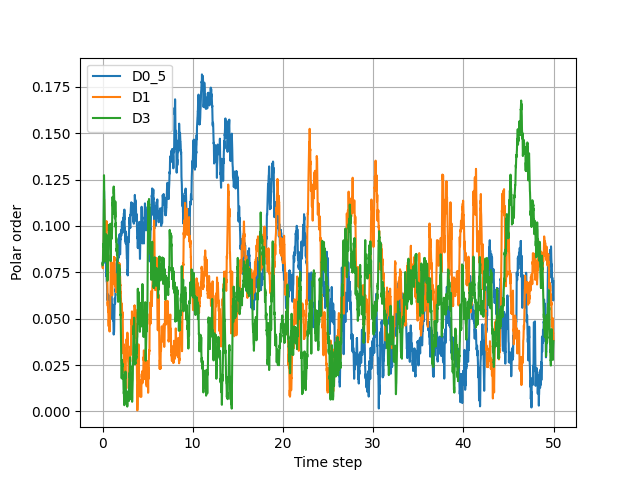
\includegraphics[width=1\textwidth]{videos/simulations/sim_D/beta0/dens_0_26/combined_polars.png}
        \caption{\footnotesize $\beta = 0$}
    \end{minipage}\hfill
    \begin{minipage}{0.49\textwidth}
        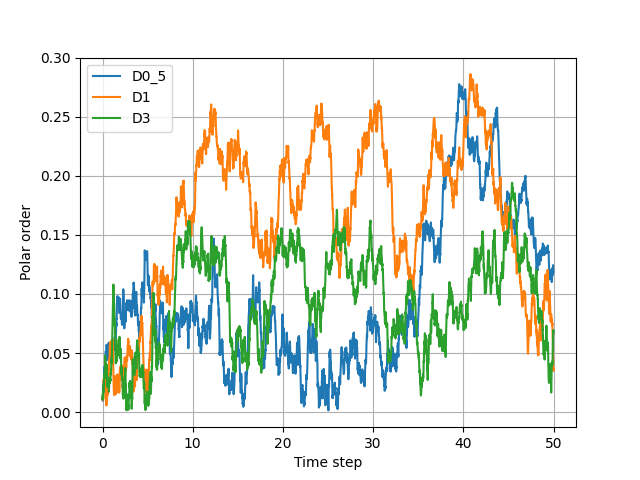
\includegraphics[width=1\textwidth]{videos/simulations/sim_D/beta1_5/dens_0_26/combined_polars.png}
        \caption{\footnotesize $\beta = 1.5$}
    \end{minipage}
\end{figure}
\begin{figure}[H]
    \begin{minipage}{0.49\textwidth}
        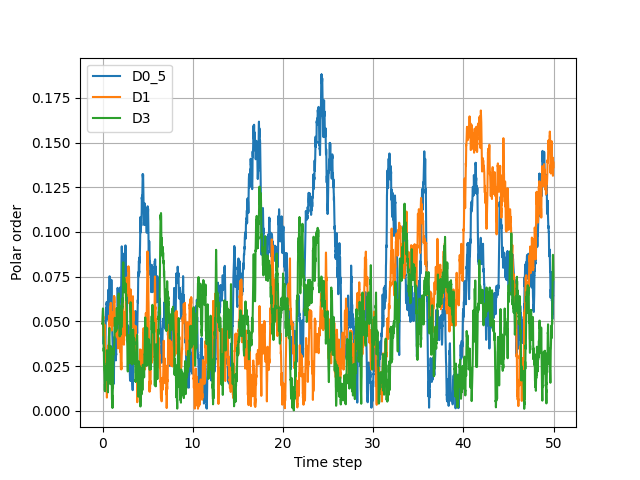
\includegraphics[width=1\textwidth]{videos/simulations/sim_D/beta3/dens_0_26/combined_polars.png}
        \caption{\footnotesize $\beta = 3$}
    \end{minipage}\hfill
    \begin{minipage}{0.49\textwidth}
        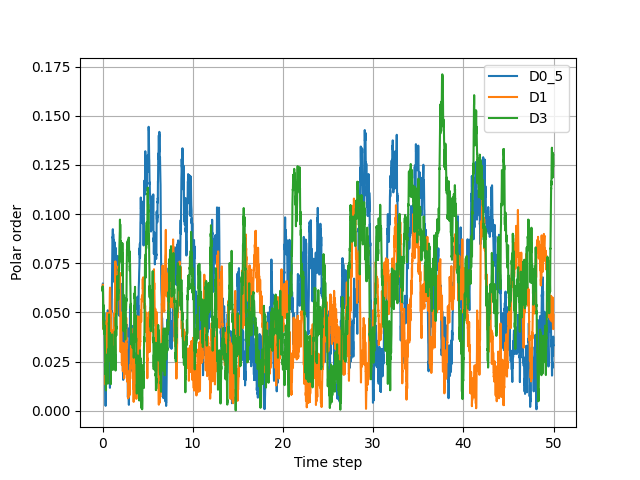
\includegraphics[width=1\textwidth]{videos/simulations/sim_D/betam1_5/dens_0_26/combined_polars.png}
        \caption{\footnotesize $\beta = -1.5$}
    \end{minipage}
\end{figure}
\begin{figure}[H]
    \centering
    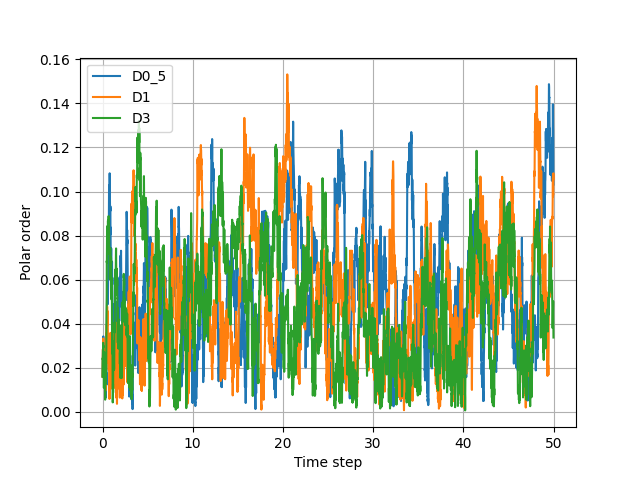
\includegraphics[width=0.5\textwidth]{videos/simulations/sim_D/betam3/dens_0_26/combined_polars.png}
    \caption{\footnotesize $\beta = -3$}
\end{figure}
The polar order parameter $v_a$ is shown over time in blue for $D = 0.5$, in orange for $D = 1$ and in green $D=3$. 
The results indicates that for $Ch_1$, no collective behaviors can be identified, as there is significant variation of $v_a$ values
between consecutive time steps. One can note that for $\beta < 0$ and $\beta = 3$, the fluctuations of $v_a$ are 
even more pronounced compared to cases where $0 < \beta < 3$.
This can be explained by the behavior seen in section \texttt{Simulation of two interacting squirmers}, for $\beta <0$, squirmers
tend to repel each other more strongly as $\beta$ decreases, while squirmers tend to attract each other
as $\beta$ increases. 

\begin{figure}[H]
    \centering
    \textbf{$Ch_2$($L_x = 4$ and $L_y = 2$), $\rho = 0.059$}\par\medskip
    \begin{minipage}{0.49\textwidth}
        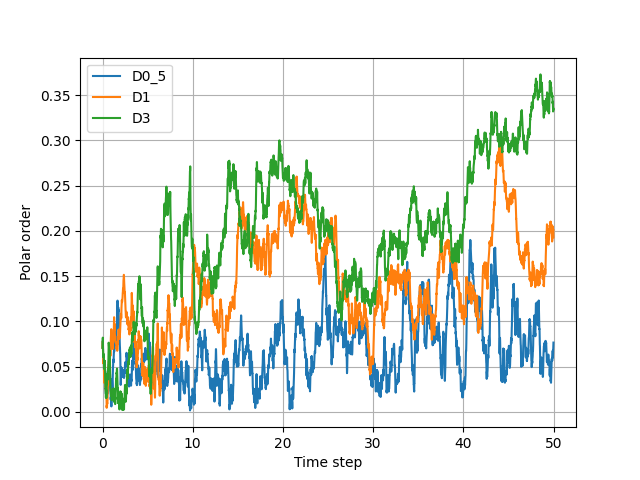
\includegraphics[width=1\textwidth]{videos/simulations/sim_D/beta0/dens_0_59/combined_polars.png}
        \caption{\footnotesize $\beta = 0$}
    \end{minipage}\hfill
    \begin{minipage}{0.49\textwidth}
        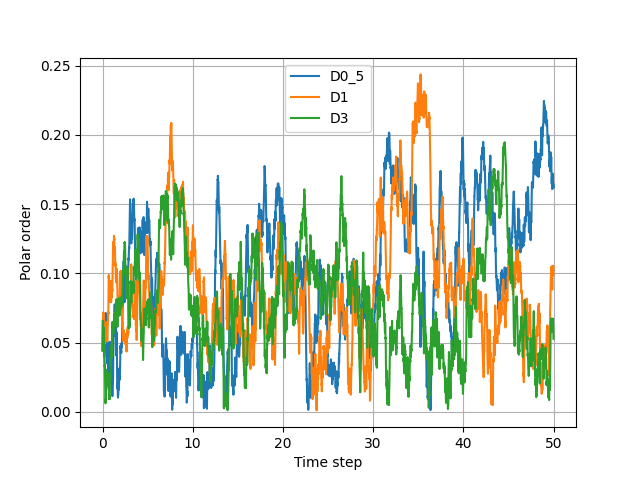
\includegraphics[width=1\textwidth]{videos/simulations/sim_D/beta1_5/dens_0_59/combined_polars.png}
        \caption{\footnotesize $\beta = 1.5$}
    \end{minipage}
    \begin{minipage}{0.49\textwidth}
        \includegraphics[width=1\textwidth]{videos/simulations/sim_D/beta3/dens_0_59/combined_polars.png}
        \caption{\footnotesize $\beta = 3$}
    \end{minipage}\hfill
    \begin{minipage}{0.49\textwidth}
        \includegraphics[width=1\textwidth]{videos/simulations/sim_D/betam1_5/dens_0_59/combined_polars.png}
        \caption{\footnotesize $\beta = -1.5$}
    \end{minipage}
\end{figure}
\begin{figure}[H]
    \centering
    \includegraphics[width=0.5\textwidth]{videos/simulations/sim_D/betam3/dens_0_59/combined_polars.png}
    \caption{\footnotesize $\beta = -3$}
\end{figure}
The results for $Ch_2$ indicates that collective behavior can be identified for $\beta = 0$ and $D = 3$, as
$v_a$ increases over time. 
A similar trend is observed for $D = 1$ and $D = 0$, although longer simulations are required to
confirm this definitively. For $\beta \neq 0$, no collective behavior are observed during the simulation. One can see that 
for $\beta \leq 0$ in $Ch_2$, the divergence of polar order parameter value between time steps is even greater
than for $\beta \leq 0$ in $Ch_1$. This can be attributed to the smaller channel size, implying more frequent interactions 
between squirmers.\\

\section{Conclusion and perspectives}
We have successfully reformulated the expressions for all forces and torques defined in the studies defined in the studies by
Brumley\cite{Brumley} and Lauga\cite{Lauga}. 
These have been implemented in a Python code to analyze their variations, either between two squirmers, between a 
squirmer and a border or between a group of squirmers.
 
Our numerical results have yielded trajectories for specific initial orientations that diverge from those reported 
by Stark \cite{Stark}.

Our simulations reveal that collective behaviors are largely absent in the $Ch_1$
channel, with significant variations in $v_a$ values, particularly for $\beta <0$ and $\beta = 3$. 
These variations can be linked to the repulsive 
and attractive interactions observed for these $\beta$ values. 
In the $Ch_2$ channel, collective behavior emerges for $\beta = 0$ and higher diffusivity, 
suggesting that a smaller channel size enhances 
interactions that promote such behavior. However, for $\beta \neq 0$, no collective behavior is observed during the simulation. 
Additionally, the increasing divergence in polar order parameter values with decreasing $\beta$ 
across both channels highlights the influence of $\beta$ on the system's dynamics.

Having thoroughly examined the interactions between squirmers and their collective behavior, 
the next phase of our research will focus on longer simulation times, higher particle densities, 
and exploring the propensity of squirmers to form clusters over time.
Another approach will involve controlling the collective behavior of squirmers using $\beta$.
\newpage

\nocite{*}
\bibliographystyle{plain}
\bibliography{bibliography/biblio}
\end{document}
